%
% A (non-exhaustive) list of TODOs:
%	- create numerical methods appendix
%	- add references
%	- display meanfield equations in appendix
% Graphs to make:
%	- comparison of 2 mode to 1 mode 
%		- NL decay of s_-
%		- Q(s_-)
%	- decay of s_+
%
%
%
%

\chapter{PhoG: Photon Gun}\label{chapter:phog}

%\section{Introduction}


In this chapter we introduce and model a device which aims to be a deterministic source of useful, highly non-classical light. The device, which we call \emph{PhoG} (``\underline{Pho}ton \underline{G}un"), uses engineered dissipation to simulate a so-called Nonlinear Coherent Loss (NCL), the steady state of which is a single-photon state. We first explore the properties of decay into a Markovian reservoir of an initial coherent state in a single-mode model, which involves one bosonic mode and a reservoir, Sec.~\ref{sec:phog_single_mode_model}. We explore the forms of dissipation required to deterministically generate useful quantum outputs, and show that although the ever-present linear (single-photon) loss prevents us from reaching perfect single-photon states, it is still possible to deterministically reach output states which are highly squeezed in photon number Sec.~\ref{sec:phog_including_loss}. These so-called sub-Poissonian states are obtained over the initial stages of the dynamics which is dominated by NCL and practically unaffected by linear loss. We then demonstrate that the NCL may be effectively simulated by more complicated models involving multiple bosonic modes and the regular Kerr nonlinearity, Secs.~\ref{sec:phog_three_mode_model}-\ref{sec:phog_multi_mode}. Finally, we demonstrate that a modification in the coupling ratio between waveguides can lead to a device which will generate quadrature entanglement between modes. Since our proposed device takes merely a coherent state input, it should prove to be a cheap and flexible source of useful quantum properties.

%\subsection{Applications of engineered loss}
\section{Introduction}

Engineered loss has, in recent years, become a powerful tool and an intensely researched field of quantum physics. Rather than simply being an enemy of the quantum state and its applications, controlled dissipation can be a helpful ally for generation, protection, and application of quantum phenomena. Furthermore, there has been renewed interest in engineered and non-standard loss mechanisms for the potential to explore new regimes of physics in which unitary and non-unitary dynamics compete or balance \cite{Ottawa2018a, Lieu2018}. For example, in Refs.~\cite{Wolinsky1988, Braun2002, Clark2003, Roghani2018} dissipation is used both to generate quantum entanglement and dissipation can even protect it \cite{Zanardi1997}. Ref.~\cite{Clark2003}, for example provides a scheme in which entanglement is generated between atoms held in distant cavities which interact solely via dissipation, while Ref.~\cite{Kimchi-Schwartz2018} allow for entanglement generation and stabilization against decay in systems of superconducting qubits. %TODO: understand how dissipation actually helps here. 

Dissipation can generate superposition states, for example the Ref.~\cite{Leghtas2015} proposes a dissipative scheme in which two-photon absorption drives a quantum state towards the Schr{\"o}dinger cat superposition state, and confines the total quantum state to states nearby to their output state. Dissipation is even found to be useful for computation. In Ref.~\cite{Verstraete2009}, Verstrate \emph{et. al.} describe how discrete systems, coupled only locally to a set of reservoirs, can allow for universal quantum computation even when the system undergoes no coherent dynamics.


The use of dissipation to enact coupling between modes also has a long history. For example, in Braun \emph{et. al.} \cite{Braun2002} two modes coupled to the same Markovian reservoir are lead to interact with each other through their correlated loss, and can generate entanglement. Such dissipative coupling may also be used to transport quantum states between separate modes in Refs.~\cite{Metelmann2015, Porras2018, Biggerstaff2016, Mogilevtsev2015, Xuereb2018}. In Ref.~\cite{Biggerstaff2016} for example it was found that dissipation can increase the rate at which a quantum state is transferred, and that dissipation can open up new types of transfer, for example between stationary eigenstates. Their scheme is particularly interesting and relevant for our work since they rely on networks of integrated waveguides. Interestingly, it is thought that such dissipatively coupled networks in Ref.~\cite{Biggerstaff2016} may even assist biological processes in nature.

\subsection{Engineering the loss}

A key requirement for enacting such dissipation-assisted protocols is that one should have precise control over both coherent and dissipative dynamics, and the system should possess the desired (engineered) dissipation while being relatively isolated from unwanted loss sources. Cavity QED has proven a useful platform \cite{Clark2003}, as have trapped ions \cite{Barreiro2011, Poyatos1996} which can allow for fine-tuning for master-equation simulation. Superconducting circuits may be another useful platform for precise and stable entanglement generation, quantum simulation and quantum error correction for computation \cite{Kimchi-Schwartz2016, Kapit2017}.

%\MT{Talk a little more about what has been achieved with control of loss, and how.} %Q: do I need to do this?

\subsection{Integrated photonic waveguides}

Each of the above systems allows for precisely controlled coupling strengths and interaction times, and crucially they allow for high effective nonlinearities to be realised. In photonic systems this is more difficult. While integrated photonic waveguides have proven useful for enacting tight-binding networks of modes, and therefore for simulating solid-state systems \cite{Mukherjee2015, Vicencio2015}, the glasses typically used have small nonlinearities and large linear (single-photon) loss. Larger effective nonlinearities can normally be obtained by choosing ultrashort pulses or by reducing the effective fiber mode area \cite{Agrawal2007, Agrawal2001}, but this may lead to other problems of confinement or higher-order dispersion processes.

Despite these issues, integrated waveguides have recently become an exciting platform with which to marry unitary and non-unitary couplings between bosonic modes, and to use these to explore interesting quantum effects. For example, recent works Refs.~\cite{Mukherjee2015, Vicencio2015} exploit collective (nonlocal) losses on the system in order to simulate a solid-state flat-band (dispersion free) state, while the integrated-waveguide platform itself allows for precise control over coupling length and strength. In any case, the generated state was found to be robust to such imperfections. Such a system may be useful for long-distance communication since it is in principle capable of propagation without dispersion.

The recent work by Mukherjee \emph{et. al.} \cite{Mukherjee2017} implements a chain of dissipatively coupled waveguides, and finds that the system acts as an effective equalizer of an input quantum state. The coupling to a common reservoir smooths out phase and amplitude fluctuations in the input state. The simultaneous action of both coherent unitary dynamics and diffusive non-unitary dynamics lead the authors to coin the term ``Coherent Diffusive Photonics" to describe photonic systems in which both unitary and diffusive action plays a key role. In the paper it was also demonstrated that the CDP platform was very robust to imperfections in both coupling strength and effective coupling length.

\subsection{Our contribution: Coherent Diffusive Photonics for quantum state generation}

\begin{figure}[htp]
\captionsetup{width=0.8\linewidth}
\centering
\includegraphics[draft=false, width=\linewidth]{phog/phog_models}
\caption{\label{fig:phog_models} Hierarchy of models of the PhoG device, from least realistic (left) to most realistic (right). We will discuss each model and relationships between them throughout the rest of this chapter. \MakeUppercase{\romannumeral 1}: Single-mode model. \MakeUppercase{\romannumeral 2}: Two-mode model. \MakeUppercase{\romannumeral 3}: Three-mode model. \MakeUppercase{\romannumeral 4}: Multi-mode model. \MakeUppercase{\romannumeral 5} Multi-mode model embedded in glass. }
\end{figure}

In this Chapter, our aim is to take the CDP platform, which consists of linear coupling and strong dissipation in an integrated waveguide network, and move it into a setting with additional realistic nonlinearity. We shall see that adding the Kerr nonlinearity, present in $\chi^{\left(3\right)}$ glasses for example, allows our CDP network to function as a deterministic generator of highly desirable quantum properties such as entanglement, photon-number squeezing and, in the ideal limit, single-photons. Our system, which we call a PhoG (\underline{Pho}ton \underline{G}un) device, is thus a passive system which is able to create highly non-classical output from a coherent state input.


Our ultimate goal in this chapter is to model a full PhoG system consisting of a network of integrated waveguides, laser-inscribed into IG$2$ glass \cite{ig2}, Fig.~\ref{fig:phog_models}~\MakeUppercase{\romannumeral 5}. The network geometry which we build up to is displayed in Fig.~\ref{fig:phog_models}~\MakeUppercase{\romannumeral 4}, and consists of two ``signal" modes (pink) coupled to each other only vicariously via a long ``tail" structure (blue) of further modes. This tail effectively simulates a reservoir over short times. In order to gain traction and insight into our system we will initially consider simpler models of increasing complexity (Fig.~\ref{fig:phog_models}, \MakeUppercase{\romannumeral 1}, \MakeUppercase{\romannumeral 2}, \MakeUppercase{\romannumeral 3}), which each explicitly consider a Markovian reservoir $R$. We will explore key effects first under the single-mode model (\MakeUppercase{\romannumeral 1}, Sec.~\ref{sec:phog_single_mode_model}) which relies on an exotic form of loss called Nonlinear Coherent Loss (NCL). This single-mode model of the PhoG device will serve to illustrate important principles which we will use going forward. 

After demonstrating that the single-mode model with NCL suitably allows for our desired states at the output, we will then show how this model may be simulated using standard linear loss, linear coupling between modes, and Kerr nonlinearity, Sec.~\ref{sec:phog_three_mode_model}. The presence of linear loss on additional modes of the system will cause our ideal single-photon output state to decay to vacuum. Despite this, strongly photon-number squeezed light is still attainable if we restrict ourselves to short evolution times. 

The requisite nonlinearity may be introduced into a real physical system by building our device in laser-inscribed waveguides in a $\chi^{\left(3\right)}$ glass, and with a future experiment in view we explore the relevant parameters in Sec.~\ref{sec:parameters}. In Sec.~\ref{sec:phog_multi_mode} we show that even these realistic parameters -- low nonlinearity and high linear loss -- are suitable to allow generation of highly sub-Poissonian output. With an experiment in mind we replace the Markovian reservoir with a long ``tail" of further bosonic modes, which effectively simulates the reservoir over the short timescales of interest, and in Sec.~\ref{sec:phog_multi_mode} we show that this multi-mode model including realistic glass paramters is still capable to create a bright output state which is strongly squeezed in photon-number.

Finally, in Sec.~\ref{sec:phog_entanglement} we show that tweaking the coupling ratio between the modes of our device can lead us to a different form of output state, and so the PhoG device can also be a deterministic source of entangled photons. We conclude in Sec.~\ref{sec:phog_outlook} with a short discussion of how the output of PhoG may be used, and an outline of necessary future work. %TODO: make sure that I do this.

Throughout the Chapter we will use several different numerical methods to model the PhoG device. The two key methods--direct integration of the master equation, and quantum monte carlo--are discussed in Appendix~\ref{appendix:phog_numerical_methods}, and a comparison between the efficiency and utility the methods is made there. Sample code which implements each method for the single-mode model (Sec.~\ref{sec:phog_single_mode_model}) may be found at Ref.~\cite{phog_code}. Throughout the Chapter will indicate when either of these methods has been used to generate specific results.


\section{Single-mode model}\label{sec:phog_single_mode_model}

\begin{figure}[htp]
\captionsetup{width=0.8\linewidth}
\centering
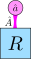
\includegraphics[width=0.2\linewidth, draft=false]{phog/single_mode}
\caption{\label{fig:phog_single_mode} A single bosonic mode, $a$, decays into a Markovian reservoir $R$ by decay operator $\hat{A}$. }
\end{figure}


Consider the single-mode model displayed in Fig.~\ref{fig:phog_single_mode} (c.f. Fig.~\ref{fig:phog_models}~\MakeUppercase{\romannumeral 1}), which consists of a single bosonic mode, $a$, decaying into a reservoir $R$ via operator $\hat{A}$. The annihilation (creation) operator for mode $a$ is $\hat{a} \left(\hat{a}^\dagger\right)$, and the density matrix containing all information about the state of the mode is $\rho_a$. This model will prove illustrative of several principles which we will develop throughout the chapter. 

Assuming that reservoir $R$ is Markovian, the evolution of mode $a$ is given by the following quantum master equation in Lindblad form \cite{Carmichael1999a, Breuer2002}


\begin{equation}\label{eqn:phog_lindblad_1}
\ddt \rho_a =  - i \left[\hat{H}, \rho_a\right] + \gamma \mathcal{L}\left[\hat{A}\right]\rho_a
\end{equation}

\noindent where we take the Hamiltonian $\hat{H} = \hbar \omega \hat{a}^\dagger \hat{a}$ ($\hbar = 1$). Equation~\ref{eqn:phog_lindblad_1} then describes the decay of an initial state $\rho_a\left(t=0\right)$ into $R$ with rate $\gamma$. The Lindbladian term $\mathcal{L}\left[\hat{A}\right]$ takes the usual form %TODO: check that I am correct to call this a Lindbladian
\begin{equation}\label{eqn:phog_lindbladian_form}
\mathcal{L}\left[\hat{A}\right]\rho_a = \hat{A}\rho_a\hat{A}^\dagger - \frac{1}{2} \hat{A}^\dagger \hat{A} \rho_a - \frac{1}{2} \rho_a \hat{A}^\dagger \hat{A}.
\end{equation}

\noindent In the remainder of this section, we examine the behaviour of an initially coherent state, $\rho_a\left(t=0\right) = \dyad{\alpha}$ with amplitude $\alpha$, as it decays into $R$. We examine several choices for decay operator $\hat{A}$ and demonstrate that suitable choices of $\hat{A}$ drive $\rho_a$ towards highly non-classical output steady-states. In Sec.~\ref{sec:A_a} we let $\hat{A} = \hat{a}$, in Sec.~\ref{sec:A_aa} we let $\hat{A} = \hat{a}^2$, and in Sec.~\ref{sec:A_ncl} we examine the behaviour of decay operators of the form $\hat{A} = \hat{a} \left(\hat{a}^\dagger \hat{a} - p\right)$ for $p \in \mathbb{N}$.



\subsection{$\hat{A} = \hat{a}$}\label{sec:A_a}
First, we consider the case $\hat{A}=\hat{a}$, which corresponds to a single-photon loss with constant rate, which we denote $\gamma$. The evolution of $\rho_a$ is described by

\begin{equation}\label{eqn:phog_lindblad_single_photon_loss}
\ddt \rho_a = \gamma\left[\hat{a}\rho_a \hat{a}^\dagger - \frac{1}{2} \hat{a}^\dagger \hat{a} \rho_a - \frac{1}{2} \rho_a \hat{a}^\dagger \hat{a}\right],
\end{equation}
where for convenience we have implicitly transformed into a rotating frame so the free Hamiltonian term $\omega \hat{a}^\dagger \hat{a}$ vanishes. Let us calculate the evolution of photon number expectation $\langle \hat{a}^\dagger \hat{a}\rangle\left(t\right)$:

\begin{align}
\ddt \langle \hat{a}^\dagger \hat{a}\rangle &= \gamma \left[ \text{Tr}\left(\hat{a}^\dagger \hat{a} \hat{a} \rho_a \hat{a}^\dagger \right) - \frac{1}{2} \text{Tr}\left(\hat{a}^\dagger \hat{a} \hat{a}^\dagger \hat{a} \rho_a\right) - \frac{1}{2} \text{Tr}\left(\hat{a}^\dagger \hat{a} \rho_a \hat{a}^\dagger \hat{a}\right)\right] \notag \\
%
&= \gamma \left[ \langle \hat{a}^\dagger \hat{a}^\dagger \hat{a}\hat{a}\rangle - \langle \hat{a}^\dagger \hat{a} \hat{a}^\dagger \hat{a}\rangle \right] \notag \\
%
&= - \gamma \langle \hat{a}^\dagger \hat{a}\rangle
\end{align}
\noindent and so
\begin{equation}\label{eqn:phog_single_photon_loss_number_expectation}
\langle\hat{a}^\dagger \hat{a} \rangle \left(t\right) = \langle \hat{a}^\dagger \hat{a}\rangle \left(0\right) e^{- \gamma t}.
\end{equation}
The photon number exponentially decays in time with decay rate $\gamma$ from its initial value. We may derive similar equations for quadrature expectations $\langle\hat{x}\rangle\left(t\right)$ and $\langle\hat{x}\rangle\left(t\right)$ and also find 
\begin{align}\label{eqn:phog_single_photon_loss_quadrature_expectation}
 \langle \hat{x}\rangle\left(t\right) &= \langle \hat{x}\rangle\left(0\right) e^{- \frac{\gamma}{2} t} \notag \\
%
 \langle \hat{p}\rangle\left(t\right) &= \langle \hat{p}\rangle \left(0\right) e^{- \frac{\gamma}{2} t}.
\end{align}

\noindent Since each of these is exponentially decaying to zero, we might guess that the steady-state of Eq.~\ref{eqn:phog_lindblad_single_photon_loss} is the vacuum $\dyad{0}$, and indeed we can deduce that this must be the case by noticing that $\ddt \rho_a = 0$ when $\rho_a$ is vacuum. In Fig.~\ref{fig:phog_lindblad_single_photon_loss}a we plot the evolution of $\langle\hat{a}^\dagger \hat{a}\rangle, \langle \hat{x}\rangle, \langle \hat{p}\rangle$ which decay towards zero, while the variances in $\hat{x}$ and $\hat{p}$ remain constant throughout the evolution. This hints that the state $\rho_a\left(t\right)$ remains a coherent state with decreasing amplitude $\alpha\rightarrow0$, until it reaches the vacuum state.

In Fig.~\ref{fig:phog_lindblad_single_photon_loss}b we plot the fidelities $\mathcal{F}$ between $\rho_a\left(t\right)$ and both the vacuum state $\dyad{0}$ and the single-photon state $\dyad{1}$. We also show fidelity between $\rho_a\left(t\right)$ and a coherent state $\dyad{\alpha^\prime}$, which is defined to have the same photon-number expectation as $\rho_a$ at all times. We observe that the fidelity to the vacuum state increases to $1$ while the fidelity to coherent state $\dyad{\alpha^\prime}=1$ always. This confirms our intuition that $\rho_a$ remains coherent $\forall t$ and that $\dyad{0}$ is the steady state. 


\begin{figure}[htp]
\captionsetup{width=0.8\linewidth}
\centering
	\begin{subfigure}{0.49\linewidth}
	\centering
	\includegraphics[draft=false, width=\linewidth]{phog/expects_a}
	\caption{}
	\end{subfigure}
	\begin{subfigure}{0.49\linewidth}
	\centering
	\includegraphics[draft=false, width=\linewidth]{phog/fidelities_a}
	\caption{}
	\end{subfigure}
\caption{\label{fig:phog_lindblad_single_photon_loss}$\hat{A} = \hat{a}$. (a) Operator expectation values calculated for state $\rho_a\left(t\right)$ as it evolves under master equation~\ref{eqn:phog_lindblad_single_photon_loss}. An initial coherent state with $\alpha=3.0$ decays to vacuum state $\dyad{0}$. Quadrature variances remain constant through time, implying that $\rho_a$ remains a coherent state throughout its evolution. This is confirmed in (b) where the fidelity between $\rho_a$ and $\dyad{\alpha^\prime}$ is demonstrated to remain $1$ for all time, while the fidelity to the vacuum state increases to $1$. The amplitude $\alpha^\prime$ is chosen to give a coherent state with equivalent photon-number expectation to $\rho_a\left(t\right)$. Horizontal gridlines displayed in black, dashed. Numerical method: direct integration.}
\end{figure}


\clearpage
\subsection{$\hat{A} = \hat{a}^2$}\label{sec:A_aa}
Next we consider a decay term $\hat{a}^2$, which describes two-photon loss into the reservoir. Our Lindblad equation is

\begin{equation}\label{eqn:phog_lindblad_two_photon_loss}
\ddt \rho_a = \gamma\left[\hat{a}^2 \rho_a \hat{a}^{\dagger 2} - \frac{1}{2} \hat{a}^{\dagger 2} \hat{a}^2 \rho_a - \frac{1}{2} \rho \hat{a}^{\dagger 2} \hat{a}^2\right]
\end{equation}
which gives the evolution of photon number expectation as 
\begin{equation}\label{eqn:aa_not_closed}
\ddt \langle \hat{a}^\dagger \hat{a}\rangle = - 2 \gamma \langle \hat{a}^\dagger \hat{a}^\dagger \hat{a}\hat{a}\rangle.
\end{equation}

\noindent This equation does not take a closed form and so we cannot yet directly calculate $\langle \hat{a}^\dagger \hat{a}\rangle\left(t\right)$. Similarly, equations for evolution of $\langle\hat{a}\rangle\left(t\right)$ require terms to the third power in $\hat{a}, \hat{a}^\dagger$, and so are also not yet closed.  We will encounter techniques later in Sec.~\ref{sec:linearization} which allow us to deal with this.

For now, let us try to deduce the steady-state of Eq.~\ref{eqn:phog_lindblad_two_photon_loss}. We observe that once again the vacuum $\dyad{0}$ must be a steady state, since then $\ddt \rho_a=0$. Surprisingly we now also have the single-photon state $\dyad{1}$, and states of the form $\dyad{0}{1}, \dyad{1}{0}$ as steady states, since these also have $\ddt \rho_a=0$. The general steady-state should be a mixture of these, and takes the form
\begin{align}\label{eqn:phog_phase_state}
&\rho_{\text{steady}} = c_1 \dyad{\psi} + c_2 \dyad{0} + c_3 \dyad{1} \notag \\
%
&\qq{with} \ket{\psi} = \frac{\ket{0} + e^{i \phi} \ket{1}}{\sqrt{2}};  \qq{} c_1, c_2, c_3 \in \mathbb{C}.
\end{align}

\noindent The state $\ket{\psi}$ is a so-called \emph{phase-state}, and it has long been known that two-photon absorption will lead to a phase state \cite{Ezaki1999} (plus additional mixing \cite{Alexanian2000, *Ezaki2000} which reduces purity). The phase $\phi$ is related to the phase of the initial coherent state. 

In Fig.~\ref{fig:phog_lindblad_two_photon_loss}a we plot the evolution of $\langle \hat{a}^\dagger \hat{a}\rangle, \langle \hat{x}\rangle, \langle \hat{p}\rangle$ and the quadrature variances. The photon number expectation no longer decays to zero as it did for $\hat{A}=\hat{a}$. %rather it decays to 0.5.
 In Fig.~\ref{fig:phog_lindblad_two_photon_loss}b we observe the fidelity between $\rho_a\left(t\right)$ and the final steady-state increases to $1$, and the coefficients of the steady state $\rho_{\text{steady}}$ are $c_1 = 0.810$, $c_2 = c_3 = 0.095$. We see therefore that two-photon loss operator induces a high degree of non-classicality in the system. We shall revisit this decay operator $\hat{a}^2$ in Sec.~\ref{sec:phog_entanglement} where we will demonstrate that it is even capable of producing entanglement between spatially separated modes of a larger system.


\begin{figure}[htp]
\captionsetup{width=0.8\linewidth}
\centering
	\begin{subfigure}{0.49\linewidth}
	\centering
	\includegraphics[draft=false, width=\linewidth]{phog/expects_aa}
	\caption{}
	\end{subfigure}
	\begin{subfigure}{0.49\linewidth}
	\centering
	\includegraphics[draft=false, width=\linewidth]{phog/fidelities_aa}
	\caption{}
	\end{subfigure}
\caption{\label{fig:phog_lindblad_two_photon_loss}$\hat{A} = \hat{a}^2$. (a) Operator expectation values for state $\rho_a\left(t\right)$ as it evolves under Eq.~\ref{eqn:phog_lindblad_two_photon_loss}. Unlike Fig.~\ref{fig:phog_lindblad_single_photon_loss}, an intially coherent state with $\alpha=3.0$ no longer decays to the vacuum state, and the final photon-number expectation is $0.5$. Quadrature variances no longer stay constant, which implies that the state is no longer a coherent state. This is confirmed in (b) where the fidelity between $\rho_a\left(t\right)$ and $\dyad{\alpha^\prime}$ is plotted. The fidelity between $\rho_a\left(t\right)$ and steady state Eq.~\ref{eqn:phog_phase_state} increases to $1$. Horizontal gridlines displayed in black, dashed. Numerical method: direct integration.} %TODO: make sure that I have defined fidelity in the introduction
\end{figure}

\iffalse
\clearpage
\subsection{$\hat{A} = \hat{a}^3$}\label{sec:A_aaa}
We might guess that the steady state of the three-photon loss term $\hat{a}^3$ is likewise a mixture of $\ket{0}, \ket{1}$ and $\ket{2}$
\begin{align}\label{eqn:phog_three_photon_loss_ss}
&\rho_{\text{steady}} = c_1 \dyad{\psi} + c_2 \dyad{0} + c_2 \dyad{1} + c_3 \dyad{2} \notag \\
%
&\qq{with} \ket{\psi} = \frac{\ket{0} + e^{i \phi}\ket{1} + e^{i \varphi}\ket{2}}{\sqrt{3}}; \; c_1, c_2, c_3, c_4 \in \mathbb{C}
\end{align}

\noindent with phases $\phi, \varphi$ in general depending on the initial coherent state $\dyad{\alpha}$. %\MT{TODO: investigate this numerically}.
Indeed, this $\rho_{\text{steady}}$ must be a steady state of the system by noting that $\hat{a}^3 \ket{\psi} = 0$ which implies $\ddt \rho_a = 0$.

We plot the evolution of fidelities between $\rho_a\left(t\right)$ evolving with decay operator $\hat{a}^3$ in Fig.~\ref{fig:phog_lindblad_three_photon_loss}, and we see the fidelity to the state in Eq.~\ref{eqn:phog_three_photon_loss_ss} increasing to $1$. \MT{additional comments.}

\begin{figure}[htp]
\centering
\includegraphics[draft=false, width=0.6\linewidth]{phog/fidelities_aaa}
\caption{\label{fig:phog_lindblad_three_photon_loss}$\hat{A} = \hat{a}^3$ (a) Fidelities between state $\rho_a\left(t\right)$ and vacuum (red), single-photon state (orange), coherent state with equivalent photon-number expectation to $\rho_a$ (green), and the two-phase state (blue). \MT{additional comments/interpretation.} Horizontal gridlines displayed in black, dashed. Numerical method: direct integration.}
\end{figure}
\fi

\clearpage
\subsection{$\hat{A} = \hat{a}\left(\hat{a}^\dagger \hat{a} - 1\right)$}\label{sec:A_ncl}
We have seen that the choice of $\hat{A}$ can give drastically different steady states of $\rho_a$,  from the uninteresting vacuum to the highly quantum and useful phase-state. We therefore wish to consider which choices for $\hat{A}$ will drive an initially coherent state to a Fock state $\dyad{n}$. 

The choice 
\begin{equation}\label{eqn:phog_A_ncl}
\hat{A} = \hat{a}\left(\hat{a}^\dagger \hat{a} - 1\right)
\end{equation}
may be interpreted as a single-photon loss at a rate which depends on photon number $\hat{n} = \hat{a}^\dagger \hat{a}$. The loss rate will go to zero when applied to state $\dyad{1}$, and so we may suspect that the single-photon state $\dyad{1}$ is a steady state of this loss mechanism.

The Lindblad equation which we solve is
\begin{equation}\label{eqn:phog_ncl_lindblad}
\ddt \rho_a = \gamma \left[ \hat{a}\left(\hat{n}-1\right) \rho \left(\hat{n}-1\right)\hat{a}^\dagger - \frac{1}{2} \rho \left(\hat{n}-1\right) \hat{n} \left(\hat{n}-1\right) - \frac{1}{2} \left(\hat{n}-1\right)\hat{n}\left(\hat{n}-1\right) \rho \right]
\end{equation}
and for convenience we have written the photon-number operator $\hat{n}$ where possible.
%The vacuum state $\dyad{0}$ also happens to be a steady-state of $\ncl$, but \MT{its coefficient remains constant, so we obtain $\dyad{1}$ in the limit of $\alpha\rightarrow \infty$}
We examine the evolution of $\rho_a$ in Fig.~\ref{fig:phog_A_ncl} and plot the evolution of photon number and quadrature expectations $\langle \hat{x}\rangle, \langle \hat{p}\rangle$ in (a). We observe a non-exponential decay of photon-number expectation to $1$, \MT{TODO: show that it is non-exponential.}
while in (b) the fidelity between $\rho_a\left(t\right)$ and $\dyad{1}$ increases to $1$. This choice of $\hat{A} = \ncl$ does indeed have a single-photon steady state. 

Even after short times $t < 0.1$ the fidelity to an equivalent coherent state has rapidly decreased, and the quadrature variances sharply increase over similar timescale. This implies a rapid increase in non-classicality of the system, which we shall explore and quantify later.

We deduce that the decay operator $\hat{a}\left(\hat{a}^\dagger \hat{a} - 1\right)$ is a useful candidate for driving our system towards the highly nonclassical single-photon state. In the remainder of this Chapter our goal will be to find a physical system which can efficiently implement this decay operator.



\begin{figure}[htp]
\captionsetup{width=0.8\linewidth}
\centering
	\begin{subfigure}{0.49\linewidth}
	\centering
	\includegraphics[width=\linewidth, draft=false]{phog/expects_ncl1}
	\caption{}
	\end{subfigure}
	\begin{subfigure}{0.49\linewidth}
	\centering
	\includegraphics[width=\linewidth, draft=false]{phog/fidelities_ncl1}
	\caption{}
	\end{subfigure}
\caption{\label{fig:phog_A_ncl}$\hat{A} = \hat{a}\left(\hat{a}^\dagger \hat{a} - 1\right)$ (a) Operator expectation values for state $\rho_a\left(t\right)$ as it evolves. An initially coherent state with $\alpha=3.0$ decays to a state with $\langle \hat{n}\rangle=1$, which we confirm as state $\dyad{1}$ by considering the fidelity in (b). Horizontal gridlines displayed in black, dashed. Numerical method: direct integration.}
\end{figure}

To gain some insight into the action of $\ncl$, let us first write the Lindblad equation~\ref{eqn:phog_ncl_lindblad} in Fock basis for density matrix element $\rho_{m, n}$
\begin{align}\label{eqn:phog_ncl_lindblad_fock}
&\ddt \rho_{m, n} = \bra{m} \ddt \rho \ket{n} \notag  \\
%
&= \gamma \left[ m \sqrt{m+1} n \sqrt{n+1} \, \rho_{m+1, n+1} - \frac{1}{2} \left(n-1\right)^2 n\, \rho_{m, n} - \frac{1}{2} \left(m-1\right)^2 m\, \rho_{m, n}\right],
\end{align}
and consider some specific matrix elements. Immediately we see that Eq.~\ref{eqn:phog_ncl_lindblad_fock} couples diagonal elements $m=n$ only to diagonal elements and so an analysis of the photon-number statistics is possible by only considering diagonal elements. We obtain, for example $\ddt \rho_{1, 1}=2 \gamma \rho_{2, 2}$ which is greater than zero, and so $\forall t$ we expect the single-photon contribution $\rho_{1,1}$ to monotonically increase, c.f. Fig.~\ref{fig:phog_A_ncl}b. 

\noindent The elements $\rho_{0, 0}, \rho_{0, 1}$ and $\rho_{1, 0}$ each give
\begin{equation}
\ddt \rho_{0,0} = 0, \qq{} \ddt \rho_{0, 1} = 0, \qq{and} \ddt\rho_{1, 0} = 0,
\end{equation}
implying that these elements are constant in time. The single-photon state requires zero in each of these elements, and so we may predict that high fidelity between $\rho_a$ and $\dyad{1}$ may only be obtained when $\rho_{0,0}\left(t=0\right)$, $\rho_{0, 1}\left(t=0\right)$, and $\rho_{1, 0}\left(t=0\right) \ll 1$. This implies, in particular, that high fidelity with $\dyad{1}$ is not obtainable for coherent states with small amplitude\footnote{The requirement of large $\alpha$ for the input coherent state is not very restrictive, and as we shall see in the next section there are additional reasons to prefer $\alpha \gg 1$}. In Fig.~\ref{fig:phog_fidelity_ncl_vs_alpha} we show this explicitly.

\begin{figure}[htp]
\captionsetup{width=0.8\linewidth}
\centering
\includegraphics[width=0.6\linewidth, draft=false]{phog/fidelities_ncl1_vs_alpha}
\caption{\label{fig:phog_fidelity_ncl_vs_alpha} The fidelity of $\rho_a\left(t\rightarrow\infty\right)$ to single-photon state $\dyad{1}$ depends on initial coherent state amplitude $\alpha$ since the density matrix elements $\rho_{0, 0}, \rho_{0, 1}$ and $\rho_{1, 0}$ are constant in time. %This helps to quantify the intuition that in a purely lossy system a state with on average less than $1$ photon could not be used to increase the photon number. Numerical method: direct integration.
}
\end{figure}




Before we move on, let us quickly explore the related operator $\hat{a}\left(\hat{a}^\dagger \hat{a} -2\right)$. Based on the above discussion we might reasonably expect the steady-state to be $\dyad{2}$, and this is indeed what we see in Fig.~\ref{fig:phog_A_ncl2}, where the fidelity to the two-photon state increases to $1$. 

We will refer to the decay described by Lindblad operator $\hat{A} = \ncl$ as \emph{nonlinear coherent loss} (NCL), since the eigenstates of the operator\footnote{The operator $\ncl$ is a specific example of $\hat{a} \hat{f}\left(\hat{n}\right)$ for operator-valued function $\hat{f}$. Glauber coherent states are obtained for the choice $\hat{f} = \hat{\mathds{1}}$.}
 $\ncl$ are known as ``nonlinear coherent states" \cite{Manko1997}, while the operator itself may be considered as the annihilation operator for a so-called $f$-deformed harmonic oscillator \cite{Filho1996}.
\begin{figure}[htp]
\captionsetup{width=0.8\linewidth}
\centering
\includegraphics[width=0.6\linewidth, draft=false]{phog/fidelities_ncl2}
\caption{\label{fig:phog_A_ncl2} $\hat{A} = \hat{a}\left(\hat{a}^\dagger \hat{a} - 2\right)$. The steady-state of this loss operator is $\dyad{2}$. The fidelity of $\rho_a$ to this two-photon state increases to $1$.}
\end{figure}



\clearpage
\section{Including loss}\label{sec:phog_including_loss}
We have seen that the nonlinear coherent loss (NCL) operator $\ncl$ is a good candidate for driving an initial coherent state towards a single photon state. Any system, therefore, which can implement the Lindblad equation~\ref{eqn:phog_lindblad_1} with decay operator $\hat{A} = \ncl$ will asymptotically and deterministically give rise to single-photon Fock states, although we have seen that fidelities close to $1$ are obtainable even at finite time, Fig.~\ref{fig:phog_A_ncl}b. 

In a realistic situation however it is unlikely that a system can be designed to implement $\ncl$ only. We must consider how the system's output states are affected by additional loss mechanisms. In an optical system the single-photon (linear) loss can never be avoided, so we will explore its effect on the nonlinear coherent loss mechanism. To do this, we modify our original Lindblad equation to include several Lindbladian terms
\begin{equation}\label{eqn:phog_lindblad_a_ncl}
\ddt \rho_a =  \gamma_1 \mathcal{L}\left[\hat{a}\right]\rho_a + \gncl \mathcal{L}\left[\ncl\right]\rho_a
\end{equation}
with $\gamma_L$ the decay rate via the single-photon loss channel $\hat{a}$, and $\gncl$ the loss rate via NCL, $\ncl$. We can immediately see that $\dyad{1}$ is only a steady-state of Eq.~\ref{eqn:phog_lindblad_a_ncl} when $\gamma_1 = 0$, in which case we revert to the analysis of Sec.~\ref{sec:A_ncl}. For all $\gamma_1 > 0$, the vacuum is the steady-state and the matrix elements $\rho_{0, 0}, \rho_{0, 1}, \rho_{1, 0}$ are no longer constant in time. 

Physically we see that the presence of linear loss leads to a degradation of the highly non-classical output states reached under NCL alone, as the additional linear loss mechanism pushes $\rho_a$ towards the vacuum. We see this explicitly in Fig.~\ref{fig:phog_A_ncl_loss}b (c.f. Fig.~\ref{fig:phog_A_ncl}), where an intially increasing fidelity with $\dyad{1}$ eventually dies away, and fidelity to the vacuum state increases to $1$. Additionally, photon number expectations decay to $0$, and an initial increase in quadrature variances decays back to the coherent state variance, Fig.~\ref{fig:phog_A_ncl_loss}a.





\begin{figure}[htp]
\captionsetup{width=0.8\linewidth}
\centering
	\begin{subfigure}{0.49\linewidth}
	\centering
	\includegraphics[width=\linewidth, draft=false]{phog/expects_ncl1_and_a}
	\caption{}
	\end{subfigure}
	\begin{subfigure}{0.49\linewidth}
	\centering
	\includegraphics[width=\linewidth, draft=false]{phog/fidelities_ncl1_and_a}
	\caption{}
	\end{subfigure}
\caption{\label{fig:phog_A_ncl_loss} NCL $\ncl$ and linear loss $\hat{a}$. Initial coherent state amplitude $\alpha=3.0$, and $\gncl=8.0$. (a) Operator expectation values. Solid: $\langle \hat{a}^\dagger \hat{a}\rangle$. The presence of linear loss $\gamma_1 > 0$ ensures that the photon number decays to $0$. Dashed: $\text{Var}\left(\hat{x}\right)$. Similarly, for $\gamma_1 > 0$ we see the variance in $x$ return to its initial value, hinting that our state is being pushed towards vacuum. (b) Fidelities of $\rho_a\left(t\right)$ against vacuum (blue), single-photon state (red) and coherent state with equivalent photon-number expectation (orange). Solid: $\gamma_1 = 0$. Dot-dashed: $\gamma_1 = 2$. Dashed: $\gamma_1 = 20$. The presence of linear loss pushes $\rho_a$ away from the single-photon state for $t > 0.1$. For $t < 0.1$ the system is dominated by NCL. Numerical method: direct integration.}
\end{figure}

%It is only for $t > 0.1$ that the fidelity decays, even for large $\gamma_1 = 20$, and for $t < 0.1$ the system seems dominated by NCL $\ncl$. 

\begin{figure}[htp]
\captionsetup{width=0.8\linewidth}
\centering
\includegraphics[width=0.49\linewidth, draft=false]{phog/max_fidelities_vs_gamma1_ncl1_and_a}
\caption{\label{fig:phog_max_fidelity} Maximum attainable fidelity between $\rho_a$ and $\dyad{1}$ at different linear loss levels $\gamma_1$. Linear loss drives $\rho_a$ towards the vacuum and destroys the quantumness of our state, but over short times the fidelity to $\dyad{1}$ appears independent of $\gamma_1$, Fig.~\ref{fig:phog_A_ncl_loss}. Here, we observe that after $\gamma_1 \approx 7.5$ the maximum attainable fidelity is practically independent of linear loss rate, while it does depends on $\alpha$. We shall exploit this later. Numerical method: direct integration.}
\end{figure}

Figure~\ref{fig:phog_A_ncl_loss}b suggests an interesting phenomenon: over short timescales the system appears to be dominated by NCL $\ncl$. Consider for example the fidelity between $\rho_a\left(t < 0.05\right)$ and $\dyad{\alpha^\prime}$ denoting a coherent state with equivalent photon-number expectation. By considering this alone, for short times the behaviour is indistinguishable from the case with $\gamma_1 = 0$. Similar reasoning applies also to the fidelities between $\rho_a\left(t < 0.1\right)$ and $\dyad{1}$, where the evolution is practically independent of $\gamma_1$ over short times.

From fidelity $\mathcal{F}\left( \rho_a\left(t<0.1\right), \dyad{0}\right)$, Fig.~\ref{fig:phog_A_ncl_loss} even suggests that $\gamma_1 \gg 0$ might help drive $\rho_a$ towards the single-photon state faster than in the $\gamma_1 = 0$ case. However we infer that loss actually is not helpful here, since after about $t=0.05$ the fidelity to $\dyad{\alpha^\prime}$ begins to increase again. This suggests that fidelity might not always be a useful measure of our desired behaviour when both nonlinear dissipation and linear loss are included.\footnote{Of course, we could have guessed this based on Fig.~\ref{fig:phog_lindblad_single_photon_loss}b as the fidelity to $\dyad{1}$ increases until $t\approx 0.25$ while the state remains completely coherent.}

We examine the maximum attainable fidelity to $\dyad{1}$ in Fig.~\ref{fig:phog_max_fidelity}. The maximum fidelity decreases with increasing $\gamma_1$, but increasing $\alpha$ appears to allow larger fidelities to be reached for the same $\gamma_1$ (c.f. Fig.~\ref{fig:phog_fidelity_ncl_vs_alpha}). We will explore this phenomenon further in Sec.~\ref{sec:phog_summary_ncl_effects}.


\subsection{Mandel parameter $Q$}
Although the fidelity has been a helpful measure for measuring the ability of our system to produce single-photons, we have observed in Fig.~\ref{fig:phog_lindblad_single_photon_loss}b a case where fidelity to the single-photon increases while $\rho_a$ remains entirely coherent. It is therefore worth considering which other measures we might use to measure progress. One such measure is the Mandel $Q$ parameter \cite{Mandel1979, Carmichael1999, Davidovich1996}
\begin{equation}\label{eqn:phog_mandelQ}
Q = \frac{\ev{\Delta\hat{n}^2}}{\ev{\hat{n}}} - 1
\end{equation}
which is written in terms of photon-number expectation $\ev{\hat{n}}$ and variance $\ev{\Delta\hat{n}^2}$. Equation~\ref{eqn:phog_mandelQ} may equivalently be written in normal order as 
\begin{equation}
Q = \frac{\ev{\hat{a}^\dagger \hat{a}^\dagger \hat{a}\hat{a}}}{\ev{\hat{a}^\dagger \hat{a}}} - \ev{\hat{a}^\dagger \hat{a}}.
\end{equation}
Intuitively, the Mandel parameter is a measure of the amount of photon-number squeezing in $\rho_a$. Coherent states have Poissonian photon-number statistics, $\ev{\Delta\hat{n}} = \ev{\hat{n}}$, and so $Q = 0$ in this case. States with $Q < 0$ have reduced photon-number variance and are known as sub-Poissonian, while states with $Q > 0$ are super-Poissonian. In the limit of zero uncertainty in photon-number, $\ev{\Delta\hat{n}} \rightarrow 0$ and so $Q \rightarrow -1$. 

Clearly, both decay operators $\ncl$ and $\hat{a}^2$ give steady-states with sub-Poissonian photon number statistics, while $\hat{a}$ gives rise to the vacuum, which is Poissonian. We will therefore seek to find parameter regimes for which the loss operators $\ncl$ or $\hat{a}^2$ give $Q<0$, even in the presence of linear loss.

%Using $Q$ as our measure to optimise has the advantage that it takes value $Q = -1$ for any Fock state and so knowledge of the steady-state of the system is not required. Additionally we do not require access to the full density matrix $\rho_a$ in order to calculate $Q$, and since $Q$ may be written entirely in terms of photon-number operator $\hat{n}$ we note that only the diagonal elements $\rho_{n, n}$ of $\rho_a$ are required. And as we observed in Sec.~\ref{sec:phog_single_mode_ncl_1}, the Lindblad equation~\ref{eqn:phog_A_ncl} couples diagonal elements to diagonal elements, which will allow for our analysis to be simplified.  \MT{Not sure where to put this paragraph or these statements.}

The effect of NCL $\ncl$ on $Q$ is displayed in Fig.~\ref{fig:phog_ncl_Q}a under several different linear loss rates $\gamma_1$. We see that the effect of NCL is indeed to drive $\rho_a$ towards a Fock state, and $Q \rightarrow -1$ for $\gamma_1 = 0$, only. For all $\gamma_1 \ne 0$ we see that $Q$ eventually returns to $0$ as the system tends towards the vacuum. However, even in this case large $\left|Q\right|$ are still obtained for finite $t$. In Fig.~\ref{fig:phog_ncl_Q} we observe that the behaviour of $Q$ over the initial evolution of $\rho_a$ is independent of linear loss rate $\gamma_1$ (c.f. Fig.~\ref{fig:phog_A_ncl_loss}b, \ref{fig:phog_max_fidelity}). This bodes well for implementation of $\ncl$ as a deterministic generator of nonclassical states, since a restriction to small times $t$ is always possible.

\begin{figure}[htp]
\captionsetup{width=0.8\linewidth}
\centering
	\begin{subfigure}{0.49\linewidth}
	\caption{}
	\includegraphics[width=\linewidth, draft=false]{phog/mandelQ_varying_gamma1}
	\end{subfigure}
	\begin{subfigure}{0.49\linewidth}
	\caption{}
	\includegraphics[width=\linewidth, draft=false]{phog/mandelQ_varying_gamma1_short_time}
	\end{subfigure}
\caption{\label{fig:phog_ncl_Q} Mandel $Q$ parameter under both NCL and linear loss. With $\gamma_1=0$, $Q \rightarrow -1$ as the system approaches $\dyad{1}$. For any $\gamma_1 > 0$, $Q\left(t\rightarrow\infty\right) \rightarrow 0$, but significant $Q < 0$ are still obtained for finite $t$. Solid: $\gncl \ne 0$. Dashed: $\gncl = 0$, i.e. just linear loss. Numerical method: direct integration. (a) and (b) show the same evolution, but (b) is displayed over a shorter timescale.}
\end{figure}

We therefore alter our goals. Since Fig.~\ref{fig:phog_ncl_Q} predicts $Q\left(t\right) > -1$ whenever $\gamma_1 \ne 0$ we will unfortunately be unable to use NCL operatpr $\ncl$ to generate single-photons. So, rather than finding a system which deterministically generates single-photon states in the long-time limit, we seek a system which will deterministically generate highly sub-Poissonian states after a specified evolution time. From now on we will take it as our goal to generate sub-Poissonian light over the initial stages of the system evolution.

We examine the best attainable $Q<0$ for a given linear loss rate $\gamma_1$, and plot in Fig.~\ref{fig:phog_ncl_best_Q_gamma1}. As we see, although the best attainable $Q$ is no longer $-1$, it varies only slightly with increasing linear loss, and even for large $\gamma_1=15$ a mandel parameter of $Q \approx -0.778$ is still attainable, while $3.2$ photons remain in the state.


\begin{figure}
\captionsetup{width=0.8\linewidth}
\centering
\includegraphics[width=0.49\linewidth, draft=false]{phog/best2_mandelQ_varying_gamma1}
\caption{\label{fig:phog_ncl_best_Q_gamma1} The best attainable value of Mandel parameter $Q$ is approximately independent of $\gamma_1$ when the loss rate is nonzero. Larger $\alpha$ allows for better $Q$ to be reached. Numerical method: direct integration ($\alpha = 2.0, 3.0, 4.0$); quantum monte carlo ($\alpha = 10.0$).}
\end{figure}

Figure~\ref{fig:phog_ncl_best_Q_gamma1} also appears to show that choosing larger initial $\alpha$ allows for smaller $Q$ to be obtained, and we saw similar effects previously in Fig.~\ref{fig:phog_max_fidelity} when considering the maximum attainable fidelity to the single-photon. While the large improvement in attainable $Q$ between $\alpha=2.0$ and $\alpha=3.0$ is primarily due to reduction in the initial $\rho_{0, 0}, \rho_{1, 0}, \rho_{0, 1}$, the improvement between $\alpha=3.0$ and $\alpha=4.0$ cannot be explained in the same way. We will explore this further using additional methods in the following sections, but for now let us briefly adopt an analytical approach. Consider the Lindblad equation describing both linear loss and NCL

\begin{equation}\label{eqn:phog_lindblad_a_ncl_2}
\ddt \rho_a = \left[ \gamma_1 \mathcal{L}\left[\hat{a}\right] + \gncl \mathcal{L}\left[\ncl\right]\right] \rho_a
\end{equation}
and expand in Fock basis
\begin{align}\label{eqn:phog_lindblad_a_ncl_fock}
\ddt \rho_{n} = - &\left[ \gamma_1 n + \gncl n \left(n - 1\right)^2 \right] \rho_n \notag \\
%
&+\left[ \gamma_1 \left(n+1\right) + \gncl \left(n+1\right) n^2 \right] \rho_{n+1},
\end{align}
where $\rho_n = \ev{\rho}{n}$. Terms in Eq.~\ref{eqn:phog_lindblad_a_ncl_fock} involving $\gncl$ are proportional to $n^3$, while terms involving $\gamma_1$ are proportional only to $n$. Therefore, for every nonzero choice of $\gamma_1, \gncl$ we see that there exists an $n$ for which the NCL dominates ($\gncl n^3 \gg \gamma_1 n$) and so Eq.~\ref{eqn:phog_lindblad_a_ncl_fock} reduces to
\begin{equation}
\ddt \rho_n \approx - \gncl n \left(n-1\right)^2 \rho_n + \gncl \left(n+1\right)n^2 \rho_{n+1}
\end{equation}
which is independent of $\gamma_1$. Thus, a sufficient increase in the initial $\ev{n}$ will compensate for the effects of linear loss, which corroborates Fig.~\ref{fig:phog_ncl_best_Q_gamma1}. We thus have an additional tool, the initial coherent state amplitude, to aid us toward generation of sub-Poissonian states via NCL.

To summarise, the inclusion of linear loss $\gamma_1$ causes our system to be driven toward the vacuum rather than a single-photon state. However, strong photon-number squeezing is obtained over the initial stages of system dynamics, Fig.~\ref{fig:phog_ncl_Q}, and is roughly independent of $\gamma_1$, Fig.~\ref{fig:phog_ncl_best_Q_gamma1}. Linear loss may further be combated \cite{Mikhalychev2013} by increasing the initial coherent state amplitude, thereby increasing $\ev{n}$, which causes NCL to dominate over the initial stages of dynamics. A strongly photon-number squeezed state is then obtained at the output by stopping the evolution at an appropriate time.


\subsection{Nonlinear decay}

Finally, let us examine behaviour of photon-number expectation $\ev{\hat{n}}$ when both NCL and linear loss are included. We have observed already, Fig.~\ref{fig:phog_A_ncl_loss}a that linear loss causes $\rho_a$ to decay to the vacuum rather than $\dyad{1}$, and so in the long-time limit we have $\ev{\hat{n}} \rightarrow 0$. We have determined however that we are primarily interested in the early stages of dynamics over which NCL dominates, and so in our system we might expect to see a signature of NCL behaviour on the photon-number expectation.

As was remarked earlier, the NCL operator $\ncl$ may be interpreted as an intensity-dependent single-photon loss, with rate proportional to $\hat{n}$. This implies that a large coherent state amplitude should give rise to quick decay of photon-number, while smaller amplitude yields smaller decay. This is in contrast to linear loss in which the decay of $\ev{n}$ is exponential with constant rate.

We vary initial coherent state amplitude $\alpha$ and plot the initial stages of dynamics in Fig.~\ref{fig:phog_ncl_NL_decay}, where we have initially set $\gamma_1=0$ in order to isolate the effects of NCL. Although each coherent state initially possesses different average photon number, after a short amount of time each state possesses the same average photon number since they have experienced different decay rates. This ``nonlinear decay'' is a key indicator of NCL \cite{Mogilevtsev2010, Shchesnovich2011}.

\begin{figure}[htp]
\captionsetup{width=0.8\linewidth}
\centering
\includegraphics[draft=false, width=0.6\linewidth]{phog/ncl_NL_decay}
\caption{\label{fig:phog_ncl_NL_decay} NCL induces intensity-dependent decay rates, and so states with initially different $\ev{\hat{n}}$ quickly decay to a level where they possess the same average photon number. This is a key demonstration of NCL. Linear loss rate $\gamma_1 = 0.0$. Numerical method: direct integration.}
\end{figure}


\subsection{Summary of NCL effects}\label{sec:phog_summary_ncl_effects}
The two signature behaviours of NCL which we have observed are
\begin{itemize}
\item $Q < 0$ Fig.~\ref{fig:phog_fig3paper}a, and 
\item Nonlinear decay of $\ev{\hat{n}}$ Fig.~\ref{fig:phog_fig3paper}b.
\end{itemize}
These are good indicators that a system is undergoing NCL. Generating the condition $Q<0$ is precisely our goal, while a system which undergoes the nonlinear decay we might reasonably expect will also generate $Q<0$. Throughout the rest of the chapter we observe these two signature behaviours in increasingly complex models, Fig.~\ref{fig:phog_models}.

Let us conclude by displaying the two signature behaviours for a system which has all three types of loss which were examined in Sec.~\ref{sec:phog_single_mode_model}, namely single-photon loss $\hat{a}$, two-photon loss $\hat{a}^2$ and nonlinear coherent loss $\ncl$. We will use parameters which in Sec.~\ref{sec:phog_three_mode_model} are demonstrated to be realistic

Specifically, we solve
\begin{equation}\label{eqn:phog_full_single_mode}
\ddt \rho_a = \left[\gamma_1 \mathcal{L}\left(\hat{a}\right) + \gamma_2 \mathcal{L}\left(\hat{a}^2\right) + \gncl \mathcal{L}\left(\ncl\right) \right] \rho_a
\end{equation}
with parameters $\gamma_2 = 0.0005$, and $\gncl = 0.002$. We allow linear loss rate $\gamma_1$ to vary, while (for $\gamma_1 >0$) it remains the dominating loss channel for the system.

\begin{figure}[htp]
\captionsetup{width=0.8\linewidth}
\centering
	\begin{subfigure}{0.49\linewidth}
	\centering
	\caption{}
	\includegraphics[width=\linewidth, draft=false]{phog/Q_paper_fig3_noloss_varalpha}
	\end{subfigure}
	\begin{subfigure}{0.49\linewidth}
	\centering
	\caption{}
	\includegraphics[width=\linewidth, draft=false]{phog/NL_decay_paper_fig3_noloss_varalpha}
	\end{subfigure}
\caption{\label{fig:phog_fig3paper} Signature behaviours of NCL in a system obeying Eq.~\ref{eqn:phog_full_single_mode} with $\gamma_2 = 0.0005$, $\gncl = 0.002$ and an initial coherent state with average photon number $\ev{\hat{n}}\left(0\right)$. (a) Generation of sub-Poissonian light, as evidenced by $Q<0$. Linear loss $\gamma_1=0$ and so the maximum value of $\left|Q\right|$ is obtained for most choices of $\alpha$, but the time taken to reach maximum $Q$ decreases as initial $\alpha$ increases. (b) Nonlinear decay of photon-number expectation $\ev{\hat{n}}$. Intensity-dependent loss causes states with large photon numbers to decay very quickly, while states with similar photon numbers experience similar decay rate. Numerical method: quantum monte carlo.}
\end{figure}

Varying $\gamma_1$ and $\alpha$, Fig.~\ref{fig:phog_fig3paper2}, we see that although linear loss $\gamma_1$ causes progressively worse values for $Q$, the dynamics are approximately independent of $\gamma_1$ over short timescales. However, for a given large $\gamma_1$, larger values of $\left|Q\right|$ can be reached by increasing the initial coherent state amplitude. Therefore, our recipe for generating non-classical states with highly sub-Poissonian photon-number statistics is to design a system which obeys Eq.~\ref{eqn:phog_full_single_mode}, and then allow an initially bright coherent state to evolve for a very short amount of time. In the limit $\gamma_1 \rightarrow 0$ this can generate states with $Q = -0.8$ (or $Q=-1$ if $\gamma_2 \rightarrow 0$ also),%TODO: understand why this is the case.
 while for all $\gamma_1 > 0$ we can force $Q \rightarrow -0.8$ by choosing $\alpha \gg 1$. The state is no longer close to a single-photon state, e.g. the best $Q$ in Fig.~\ref{fig:phog_fig3paper2}b occurs when the state with initially $\ev{\hat{n}}=700$ has reduced to $\ev{\hat{n}} = 285$, and so the output state is both bright and highly sub-Poissonian. %We shall discuss possible applications of such a state in Sec.~\MT{X}.

\begin{figure}[htp]
\captionsetup{width=0.8\linewidth}
\centering
	\begin{subfigure}{0.49\linewidth}
	\centering
	\caption{}
	\includegraphics[width=\linewidth, draft=false]{phog/Q_paper_fig3_alpha500_vargamma1}
	\end{subfigure}
	\begin{subfigure}{0.49\linewidth}
	\centering
	\caption{}
	\includegraphics[width=\linewidth, draft=false]{phog/Q_paper_fig3_gamma1200_varalpha}
	\end{subfigure}
\caption{\label{fig:phog_fig3paper2} Evolution of the Mandel $Q$ parameter as $\gamma_1$ and $\alpha$ are varied in a system obeying Eq.~\ref{eqn:phog_full_single_mode} with $\gamma_2 = 0.0005$, $\gncl = 0.002$ and an initial coherent state with average photon number $\ev{\hat{n}}\left(0\right)$. (a) Constant $\ev{\hat{n}}\left(0\right) = 500$ photons and varying linear loss $\gamma_1$. Larger $\gamma_1$ causes progressively smaller values of $\left|Q\right|$ to be obtained, c.f. Fig.~\ref{fig:phog_ncl_best_Q_gamma1}, although the dynamics are practically independent of $\gamma_1$ for small times. (b) Constant $\gamma_1 = 200$. Even with large linear loss, larger $\left|Q\right|$ may be obtained by starting with a brighter coherent state (larger $\ev{\hat{n}}\left(0\right)$). Numerical method: quantum monte carlo.}
\end{figure}



\clearpage
\section{Three-mode model}\label{sec:phog_three_mode_model}
Having analysed the single-mode model in detail, and demonstrated that the NCL operator $\ncl$ is a good candidate for deterministic generation of highly non-classical states even in the presence of two-photon loss and strong linear loss, we must turn to consider whether such an NCL operator can be effectively realised in practice. In this section we will demonstrate that $\ncl$ may be effectively simulated in a three-mode system via a combination of strong linear loss, linear coupling between multiple modes, and the Kerr nonlinearity. Our starting point is the three-mode model depicted in Fig.~\ref{fig:phog_three_mode} in which two bosonic modes, $a$ and $b$, are coupled to a third, $c_0$, which decays into a Markovian reservoir $R$ with decay rate $\gamma_c$. 

\begin{figure}[htp]
\centering
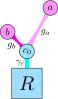
\includegraphics[width=0.3\linewidth, draft=false]{phog/three_mode}
\caption{\label{fig:phog_three_mode} Three-mode model of PhoG device. Two bosonic modes, $a$ and $b$, are each coupled to a third mode, $c_0$. Mode $c_0$ is then strongly coupled to Markovian reservoir $R$ via linear loss $\left(\hat{A} = \hat{a}\right)$ with decay rate $\gamma_c$. }
\end{figure}

The Lindblad equation describing this three-mode model is
\begin{equation}\label{eqn:phog_lindblad_three_mode_model}
\ddt \rho_3 = - i \left[ \hat{H}_3, \rho_3\right] + \left[ \gamma_1 \mathcal{L}\left[\hat{a}\right] + \gamma_1 \mathcal{L}\left[\hat{b}\right] + \gamma_c \mathcal{L}\left[\hat{c}_0\right]\right] \rho_3
\end{equation}
where the subscript $3$ denotes that we are dealing with this three-mode model. We have additionally assumed that modes $a$ and $b$ to be coupled to independent Markovian reservoirs with rate $\gamma_1$ which models the conventional linear loss. The Hamiltonian is taken to be $\hat{H}_3 = \hat{H}_3^{\text{int}} + \hat{H}_3^{\text{Kerr}}$, where
\begin{align}\label{eqn:phog_three_mode_hamiltonian}
&\hat{H}_3^{\text{int}} = g_a \hat{a}^\dagger \hat{c}_0 + g_b \hat{b}^\dagger \hat{c}_0 + \hc \notag \\
%
&\hat{H}_3^{\text{Kerr}} = \frac{U}{2} \sum_{x} \hat{x}^\dagger \hat{x}^\dagger \hat{x} \hat{x} \qq{with} \hat{x} \in \left\{\hat{a}, \hat{b}, \hat{c}_0\right\}.
\end{align}
The interaction Hamiltonian $\hat{H}_3^{\text{int}}$ describes linear coupling between modes, while the Kerr Hamiltonian $\hat{H}_3^{\text{Kerr}}$ describes the self-Kerr interaction (self-phase modulation) % Check that these are indeed equivalent
on each mode. This Hamiltonian may be realised, for example, by evanescently coupled waveguides in a $\chi^{\left(3\right)}$ glass. The constant $U$ is the Kerr nonlinear interaction constant, and we will relate this to glass properties in Sec.~\ref{sec:parameters}, below.

The three-mode model Eq.~\ref{eqn:phog_lindblad_three_mode_model}, while a physically useful starting point for building a system which accurately simulates NCL, is currently too difficult to analyse, either analytically or using the numerical methods which proved useful for the single mode model in Secs.~\ref{sec:phog_single_mode_model},~\ref{sec:phog_including_loss} (see Appendix~\ref{appendix:phog_numerical_methods}). 

We may reduce the complexity of Eq.~\ref{eqn:phog_lindblad_three_mode_model} by assuming that the decay rate $\gamma_c$ of mode $c_0$ into the reservoir $R$ is large enough that mode $c_0$ completely decays on a much faster timescale than modes $a, b$. This will allow for adiabatic elimination of mode $c_0$ via the methods described in Appendix.~\ref{appendix:adiabatic_elimination}. We identify
\begin{align}
&H^{\left(0, 0\right)} = \frac{U}{2} \sum_{x \in \left\{a, b\right\}} x^{\dagger 2} x^2 \notag \\
%
&H^{\left(0, 1\right)} = g_a a^\dagger c_0 + g_b b^\dagger c_0 \notag \\
%
&H^{\left(0, 2\right)} = 0
\end{align}
and so, substituting into Eq.~\ref{eqn:adiabatic_elimination}, we arrive at
\begin{equation}\label{eqn:phog_two_mode_model_deriv}
\ddt \rho_2 = - i \left[\frac{U}{2} \sum_{x \in \left\{a, b\right\}} x^{\dagger 2} x^2, \rho_2\right] + \frac{4 G^2}{\gamma_c} \mathcal{L}\left[\frac{g_a a + g_b b}{G} \right]\rho_2 + \gamma_1 \left(\mathcal{L}\left[a\right] + \mathcal{L}\left[b\right]\right)\rho_2,
\end{equation}
where $G = \sqrt{g_a^2 + g_b^2}$. The three-mode model has been reduced to a two-mode system involving only modes $a, b$. Introducing the following collective symmetric and antisymmetric modes

\begin{align}\label{eqn:phog_rotation}
\hat{s}_+ &= \frac{1}{G} \left(g_a \hat{a} + g_b \hat{b}\right) \qq{symmetric}  \notag \\
%
\hat{s}_- &= \frac{1}{G} \left(g_a \hat{b} - g_b \hat{a}\right) \qq{antisymmetric}
\end{align}
and rewriting Eq.~\ref{eqn:phog_two_mode_model_deriv} in terms of these new modes we arrive at the final equation for our two-mode model
\begin{equation}\label{eqn:phog_lindblad_two_mode_model}
\ddt \rho_2 = - i \left[ \hat{H}_2, \rho_2 \right] + \left[ \gamma_1 \mathcal{L}\left[\hat{s}_-\right] + \left(\Gamma + \gamma_1\right) \mathcal{L}\left[\hat{s}_+\right] \right] \rho_2
\end{equation}
where the subscript $2$ denotes that each quantity is for this two-mode model, and we have defined $\Gamma = 4 G^2 / \gamma_c$. The Hamiltonian $\hat{H}_2$ takes the form $\hat{H}_2 = \hat{H}_2^{\text{self}} + \hat{H}_2^{\text{int}}$, with
\begin{align}
&H_2^{\text{self}} = \varsigma_1\left(n_+^2 + n_-^2\right) + \varsigma_2 n_+ n_- + \varsigma_3\left(n_+ + n_-\right) \notag \\
%
&H_2^{\text{int}} = \varsigma_4 \left(s_+^\dagger s_-\right)^2 + \varsigma_5 s_+^\dagger s_- \left(n_- - n_+ - 1\right) + \hc
\end{align}
where $n_{\pm} = s_{\pm}^\dagger s_\pm$. Our $\varsigma$ coefficients are
\begin{align}
&\varsigma_1 = \frac{U}{2 G^4} \left(g_a^4 + g_b^4\right), \; \varsigma_2 = \frac{4 U}{G^4} \left(g_a g_b\right)^2, \notag \\
%
&\varsigma_3 = \frac{\varsigma_2}{4} - \frac{U}{2}, \; \varsigma_4 = \frac{\varsigma_2}{4}, \; \varsigma_5 = \frac{U}{G^4} g_a g_b \left(g_a^2 - g_b^2\right).
\end{align}
The two-mode model obeying Eq.~\ref{eqn:phog_lindblad_two_mode_model} is depicted in Fig.~\ref{fig:phog_two_mode_model} where we see that mode $s_+$ decays into reservoir $R$ with decay rate $\Gamma + \gamma_1$. In the absence of linear loss, $\gamma_1=0$, mode $s_-$ will decay only vicariously through $s_+$, and the coupling between modes is proportional to nonlinearity parameter $U$. In a linear system, $U = 0$, the antisymmetric mode $s_-$ will not decay and so we identify it as the dark mode of the system, which is considered further e.g. in Ref.~\cite{Delanty2012}.


\begin{figure}[htp]
\centering
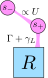
\includegraphics[width=0.3\linewidth, draft=false]{phog/two_mode}
\caption{\label{fig:phog_two_mode_model} Two-mode model of the PhoG device. Having adiabatically eliminated mode $c_0$ from the three-mode model (Fig.~\ref{fig:phog_three_mode}) and rotated to collective basis $s_-, s_+$ using Eqs.~\ref{eqn:phog_rotation} we see that mode $s_-$ will only decay into $R$ by first decaying into $s_+$. The linear coupling between $s_-$ and $s_+$ is proportional to $U$, and so for a linear system $U=0$ mode $s_-$ cannot decay into $R$. Decay rate $\Gamma = 4 G^2 / \gamma_1$.}
\end{figure}


However, even two bosonic modes are computationally very challenging to simulate when large photon numbers are required\footnote{For example, we shall note in Appendix~\ref{appendix:phog_numerical_methods} that a coherent state may be accurately modelled on a Hilbert space size $2 \lceil \alpha^2 \rceil$ without adverse effects due to Hilbert space truncation. Initial $\ev{\hat{n}} = 700$, required in Fig.~\ref{fig:phog_fig3paper2}b to give large negative $Q$, will require a Hilbert space size $\dims > 1400$ on each mode, and so a total Hilbert space size of $1400 \times 1400 = 1960000$. This is challenging to implement.}, although we shall encounter approximation methods in Sec.~\ref{sec:linearization} which help us to deal with this. 

We thus seek to adiabatically eliminate mode $s_+$ from the system, which will leave us with an equation for $s_-$ only. Let us assume that the decay rate $\Gamma + \gamma_1$ is the dominating decay rate of the two-mode model, and that mode $s_+$ decays to its steady state much quicker than the typical timescale of the dynamics of $s_-$. Then applying the adiabatic elimination method described in Appendix~\ref{appendix:adiabatic_elimination} we identify

\begin{align}\label{eqn:phog_single_mode_deriv_adiabatic}
H^{\left(0, 0\right)} &= \varsigma_1 n_-^2 + \varsigma_3 n_- \notag \\ 
%
H^{\left(0, 1\right)} &= \varsigma_5 s_-^\dagger n_- \notag \\
%
H^{\left(0, 2\right)} &= \varsigma_4 s_-^{\dagger 2}
\end{align}
and so

\begin{equation}\label{eqn:phog_single_mode_deriv}
\ddt \rho_1 = - i \left[\hat{H}_1, \rho_1\right] + \left\{\gamma_1 \mathcal{L}\left[s_-\right] + \gamma_2 \mathcal{L}\left[s_-^2\right] + \gncl \mathcal{L}\left[\ncl\right] \right\}\rho_1
\end{equation}
where we have used the commutator to write $n_- s_- \rightarrow \ncl$. The decay rates are
\begin{equation}\label{eqn:phog_single_mode_decay_rates}
\gamma_2 = \frac{4 U^2 \left(g_a g_b\right)^4}{G^8 \left(\Gamma + \gamma_1\right)} \qq{and} \gncl = \frac{4 U^2 \left(g_a g_b\right)^2}{G^8 \left(\Gamma + \gamma_1\right)}\left(g_a^2 - g_b^2\right)^2.
\end{equation}

\noindent We see that Eq.~\ref{eqn:phog_single_mode_deriv} matches Eq.~\ref{eqn:phog_full_single_mode} except for the addition of the Hamiltonian $\hat{H}_1 = H^{\left(0, 0\right)}$ in Eqs.~\ref{eqn:phog_single_mode_deriv_adiabatic} which does not affect the photon-number statistics. 



The effective decay rates $\gamma_2, \gncl$ in this single-mode model explicity depend on coupling constants $g_a, g_b$ (Fig.~\ref{fig:phog_three_mode}, Eq.~\ref{eqn:phog_three_mode_hamiltonian}). We see for example that in the limit of symmetric coupling $g_a = g_b$, $\gncl = 0$ and there will be no NCL for mode $s_-$. Large $\gncl$ can be obtained however for strong asymmetry $g_a \gg g_b$ or $g_b \gg g_a$. 

Since it is NCL which drives $\rho$ most effectively towards highly sub-Poissonian states we will seek to maximise $\gncl$. We fix $G = \sqrt{g_a^2 + g_b^2}$ and define $g_a = x G, g_b = \sqrt{1-x^2}G$ for $0 < x < 1$. Substituting these couplings into our equation for $\gncl$ we see that
\begin{equation}
\gncl = \frac{- 4 U x^2 \left(1 - 2 x^2\right)^2 \left(-1 + x^2\right)}{\Gamma + \gamma_1}.
\end{equation}
We proceed by setting $\frac{\mathrm{d}}{\mathrm{d}x} \gncl = 0$, which yields
\begin{equation}
x = \frac{\sqrt{2 + \sqrt{2}}}{2}
\end{equation}
as the only solution\footnote{Note that $x = 1/\sqrt{2}$ is the only other solution with $0 < x < 1$. This choice of $x$ will yield symmetric coupling $g_a = g_b$ and hence $\gncl=0$. We will return to this scenario in Sec.~\ref{sec:phog_entanglement}.} $0 < x < 1$ which will yield a nonzero $\gncl$. So, the optimum choice for $g_a, g_b$ is
\begin{equation}\label{eqn:phog_gagb_optimal}
g_b = \left(\sqrt{2} - 1\right)g_a.
\end{equation}
Taking this optimal choice,
\begin{equation}\label{eqn:phog_gamma3_optimal}
\gamma_2 = \frac{U^2}{16\left(\Gamma + \gamma_1\right)} \qq{and} \gncl = \frac{U^2}{4 \left(\gamma_1 + \Gamma\right)},
\end{equation}

%%%%%%%%%%%%%%%%%%%%%%%%%%%%%%%%%%%%%%%%%%%%%%%%%%%%%%%%%%%%%%%%
\noindent and we are finally able to give motivation for the choices of $\gamma_2=0.0005, \gncl=0.002$ used in Sec.~\ref{sec:phog_summary_ncl_effects} as the decay rates given by Eq.~\ref{eqn:phog_gamma3_optimal} when $\Gamma = 432 g$, $U = 2 g$, $\gamma_1 = 0$ and $g$ is a dimensionless scaling parameter which we here take to be $1$. Altering $g$ will only serve to re-scale the time axis of Figs.~\ref{fig:phog_fig3paper},~\ref{fig:phog_fig3paper2} but the qualitative dynamics will remain unchanged. 

To summarise, we have reduced the three-mode model (Eq.~\ref{eqn:phog_lindblad_three_mode_model}, Fig.~\ref{fig:phog_three_mode}) to a single-mode model (Eqs.~\ref{eqn:phog_full_single_mode}
,~\ref{eqn:phog_single_mode_deriv}, Fig.~\ref{fig:phog_single_mode}) via sequential adiabatic eliminations of modes $c_0$ and $s_+$, which rapidly decayed into reservoir $R$. In essence, the behaviour of the antisymmetric collective mode $s_-$ in the three-mode model simulates behaviour of a single mode undergoing nonlinear coherent loss, two-photon loss and single-photon loss, which were all considered in Secs.~\ref{sec:phog_single_mode_model},~\ref{sec:phog_including_loss}. The combination of Kerr nonlinearity, linear coupling and single-photon loss allows for the effective NCL decay operator to be constructed.

We demonstrate in Figs.~\ref{fig:phog_three_mode_single_mode_comparison},~\ref{fig:phog_two_mode_single_mode_comparison} that both the three-mode model and the two-mode model do  indeed give rise to the same behaviour as the single-mode model. Considering the two-mode model (Fig.~\ref{fig:phog_two_mode_single_mode_comparison}a) we see that initially mode $s_-$ does not have rapid decay. This is because mode $s_+$ is populated (Fig.~\ref{fig:phog_two_mode_single_mode_comparison}b). However, once $s_+$ begins to decay, we observe good agreement between two-mode and single-mode model. The two-mode model exhibits behaviours signature to NCL.


\begin{figure}[htp]
\centering
\includegraphics[width=0.49\linewidth, draft=false]{phog/PhoG-fig8}
\caption{\label{fig:phog_three_mode_single_mode_comparison}
Evolution of Mandel parameter (a) and mean photon number (b) of the antisymmetric mode $s_-$ computed via the three-mode model (solid lines) and the single-mode model (dots) for parameters: $g_b / g_a = \sqrt{2} - 1$, $U = 0.012 g_b$, $\gamma_c = 6.04 g_b$, and $\gamma_1 = 0.0$. \emph{Picture credit: Anton Sakovich in Ref.~\cite{Thornton2019a}}. Numerical method: quantum monte carlo (three-mode model); direct integration of Eq.~\ref{eqn:phog_lindblad_a_ncl_fock} (single-mode model)}
\end{figure}

\begin{figure}[htp]
\centering
	\begin{subfigure}{0.49\linewidth}
	\caption{}
	\includegraphics[width=\linewidth, draft=false]{phog/NL_decay_two_mode_one_mode_comparison}
	\end{subfigure}
	\begin{subfigure}{0.49\linewidth}
	\centering
	\caption{}
	\includegraphics[width=\linewidth, draft=false]{phog/two_mode_model_splus}
	\end{subfigure}
\caption{\label{fig:phog_two_mode_single_mode_comparison} (a) Comparison of nonlinear decay for single-mode model (solid) and two-mode model (dashed) with varying input $\ev{\hat{n}_-}$. Input $\ev{\hat{n}_+} = 0$, optimal couplings $g_a, g_b$, $\gamma_1 = 10.0$ and otherwise equivalent parameters to Fig.~\ref{fig:phog_fig3paper}. Finite (nonzero) decay time (b) of mode $s_+$ means that the adiabatic elimination of $s_+$ is not yet valid for $t \approx 0$. Otherwise, there is good agreement between models once $s_+$ has begun to decay, and the two-mode model exhibits the same signature behaviours of NCL.}
\end{figure}

\clearpage
\section{Realistic parameters}\label{sec:parameters}

Let us consider how the analysis we have performed so far connects to real parameters of a physical system which capable of implementing the PhoG device. We have in mind a network of waveguides laser-inscribed into IG$2$ class \cite{ig2}, using methods similar to the recent work Ref~\cite{Mukherjee2017}. Our envisioned system is depicted in Fig.~\ref{fig:phog_realistic}.

\begin{figure}[htp]
\centering
\includegraphics[draft=false, width=0.49\linewidth]{phog/phog3D}
\caption{\label{fig:phog_realistic} $3$D representation of finished PhoG device. Waveguides are laser-inscribed into IG$2$ glass and allow for NCL to be simulated.}
\end{figure}

We must consider two new things: (i) realistic glass parameters and how they influence constants which enter into our Lindblad equations~\ref{eqn:phog_lindblad_three_mode_model},~\ref{eqn:phog_lindblad_two_mode_model},~\ref{eqn:phog_single_mode_deriv}; (ii) simulation of a Markovian reservoir $R$ by a ``tail" of additional bosonic modes. We consider (i) in this section, and (ii) in Sec.~\ref{sec:phog_multi_mode}.

We will derive realistic parameters in this section, and they will be used in Sec.~\ref{sec:phog_multi_mode} to show that the desired signature behaviours are still observed. These order-of-magnitude calculations are intended to illustrate feasibility of our device in real glass, and ideally many of the parameters must be measured experimentally on the device itself.

One important quantity to estimate is the Kerr nonlinearity parameter $U$ which is used in our Hamiltonians. To do so, we will follow the analyses put forth in Refs.~\cite{Drummond1980, Imoto1985, Kitagawa1986}, and assume that a pulse of finite length $L_\eff$ propagates through a waveguide with $L$, such that $L \gg L_\eff$. The waveguide in $\chi^{\left(3\right)}$ glass is assumed to have no dispersion and the pulse shape does not change. We consider only the changes of the quantum state of the pulse caused by nonlinearity, linear loss and nonlinear phase changes\footnote{We will briefly discuss relaxation of these conditions in Sec.~\ref{sec:outlook}}. %Outlook section where I will discuss pulses briefly

The Kerr nonlinearity parameter may be written as 
\begin{equation}
U = 2 \hbar \frac{\omega^2}{V_\eff} \frac{n_2}{n_\eff}
\end{equation}
which is derived e.g. in Refs.~\cite{Imoto1985, Kitagawa1986, Drummond1980} either in terms of nonlinear refractive index parameter $n_2$ or third-order susceptibility tensor $\chi^{\left(3\right)}$. $V_\eff$ is the effective mode area which we take to be $V_\eff \sim A_\eff L_\eff$, with $A_\eff$ the transverse mode area. We take the effective refractive index of the waveguide mode to be $n_\eff \approx 2.5$ which is typical for IG$2$ glass \cite{ig2}. IG$2$ also has $n_2 \sim 3 \times 10^{-18} \text{W}^{-1} \text{m}^2$ \cite{Demetriou2017, Wang2014}. %\MT{comment about suitability of each of these assumptions. How much are the numbers likely to vary in the final device?} 

The effective mode area is uncertain, and so as an upper bound we take $A_\eff$ to be the area of the waveguide which is on the order of $10^{-12}\text{m}^2$ as in Ref.~\cite{Mukherjee2017} for similar laser-inscribed waveguides  capable of supporting large pulse energies. Taking for example $A_\eff = 120\times10^{-12} \text{m}^2$, for a $100$~fs pulse at $1064$~nm we calculate $U \approx 8.5\times 10^{-8}$. This certainly seems feasible, and we may expect the final values of $U$ to even increase in a finished device owing to reduction in $A_\eff$ (e.g. in Ref.~\cite{Mukherjee2017} the waveguides are approximately $4 \mu\text{m} \times 4 \mu\text{m}$.) Evolution under this $U = 8.5\times10^{-8}$ is modelled in Sec.~\ref{sec:phog_multi_mode}. We should stress however that the specific value of $U$ must be measured on a final physical device, and the values in this section are order-of-magnitude estimates only.

%\MT{Calculation of $\gamma_1$? Calculation of approximate coupling constants?}




%\clearpage
\section{Multi-mode model}\label{sec:phog_multi_mode}
In the previous sections we have demonstrated that the three-mode model considered in Sec.~\ref{sec:phog_three_mode_model} accurately simulates NCL and allows for deterministic generation of sub-Poissonian light over the initial stages of the dynamics. A natural next question to ask is ``how might we implement such a model?". %\MT{add a little overview of some of the literature.}

One approach which was successfully demonstrated in Ref.~\cite{Mukherjee2017} is to replace the Markovian reservoir $R$ with a ``tail" of further bosonic modes. %This mirrors a common numerical technique \MT{cite a bunch of stuff} which is regularly used to numerically simulate non-Markovian reservoirs. 
Here we adopt this replacement in order to implement the system in laser-inscribed waveguides, identically to Ref.~\cite{Mukherjee2015, Mukherjee2017}.

We therefore wish to analyse the multi-mode model of the PhoG device, Fig.~\ref{fig:phog_multi_mode} in which two "signal" modes are linearly coupled to a "tail" of further modes. The intra-tail coupling $g_c$ should be chosen to mimic the effect of reservoir $R$. We will solve this model and compare it to the models used previously in order to demonstrate agreement between these approaches. %Gotta mention later in my graphs and analysis that I have chosen the best $g_c$.
The Lindblad master equation describing the multi-mode system is

\begin{equation}\label{eqn:phog_multi_mode}
\ddt \rho = - i \left[\hat{H}, \rho\right] + \gamma_1 \left[\mathcal{L}\left[\hat{a}\right] + \mathcal{L}\left[\hat{b}\right] + \sum_{j=0}^N \mathcal{L}\left[\hat{c}_j\right] \right] \rho
\end{equation}
with $\hat{H} = \hat{H}^{\text{int}} + \hat{H}^{\text{Kerr}}$, and
\begin{align}
&\hat{H}^{\text{int}} = g_a \hat{a}^\dagger \hat{c}_0 + g_b \hat{b}^\dagger \hat{c}_0 + \sum_{j=1}^N g_j \hat{c}_{j-1}^\dagger \hat{c}_j + \hc \notag \\
%
&\hat{H}^{\text{Kerr}} = \frac{U}{2} \sum_{x \in \left\{a, b, c_j\right\}} \hat{x}^\dagger \hat{x}^\dagger \hat{x} \hat{x}, \qq{} j = 0, 1, \dots, N
\end{align}
with Kerr nonlinearity constant $U$, total number of tail modes $N$, and couplings $g_a, g_b, g_c$. We cannot hope to numerically simulate Eq.~\ref{eqn:phog_multi_mode} over the necessary parameter regimes of large input $\alpha$ and large number of modes\footnote{Even taking each mode as a qubit cannot help, as the total Hilbert space size is $2^{N}$ which is intractable for $N$ large.}, $N$. For the multi-mode model the only decay route into a Markovian reservoir is via linear loss $\gamma_1$, and so we require the tail to be long enough that state which has initially decayed into the tail cannot return to the signal modes over the timescales of interest. We are therefore trapped in the unfortunate scenario of having to make predictions of the behaviour of a large number of coupled modes, with strong nonlinearity and a necessarily large Hilbert space size of each mode. 

\begin{figure}[htp]
\centering
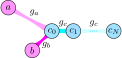
\includegraphics[width=0.6\linewidth, draft=false]{phog/multi_mode}
\caption{\label{fig:phog_multi_mode} Multi-mode model of the PhoG device (c.f. Fig.~\ref{fig:phog_models}~\MakeUppercase{\romannumeral 4}) in which the Markovian reservoir $R$ from the three-mode model (Fig.~\ref{fig:phog_three_mode}) is replaced by a long ``tail" of additional bosonic modes.}
\end{figure}

To proceed we will consider two related approaches to approximate the system Eq.~\ref{eqn:phog_multi_mode}: a meanfield approach (Sec.~\ref{sec:meanfield}) and a quantum linearization approach (Sec.~\ref{sec:linearization}). Each of these techniques will give us a set of coupled differential equations for expectations of quantum operators. The number of equations scales only polynomially\footnote{Rather than the exponential scaling of the Lindblad master equation~\ref{eqn:phog_multi_mode}.} in $N$ and so is much more manageable than the numerical methods considered in Appendix~\ref{appendix:direct_integration},~\ref{appendix:monte_carlo} and used in previous sections.

\subsection{Meanfield approach}\label{sec:meanfield}
To illustrate the first of these approaches, let us use our master equation~\ref{eqn:phog_multi_mode} to find an equation for expectation $\ev{\hat{a}}$ of mode $a$. We see that
\begin{equation}
\ddt \ev{\hat{a}}\left(t\right) = \text{Tr}\left( \hat{a} \ddt \rho\right)
\end{equation}
and so
\begin{equation}\label{eqn:phog_meanfield_deriv}
\ddt \ev{\hat{a}}\left(t\right) = - i g_a \ev{\hat{c}_0} - i \frac{U}{2} \ev{\hat{a}^\dagger \hat{a}\hat{a}} - \frac{\Gamma}{2} \ev{\hat{a}}
\end{equation}
which is an exact differential equation for $\ev{\hat{a}}$ in terms of first- and third-order expectations. Analogously, equations for second-order terms such as $\ev{\hat{a}\hat{a}}$ or $\ev{\hat{a}^\dagger \hat{a}}$ will involve second- and fourth-order expectations. As we noted in the discussion around Eq.~\ref{eqn:aa_not_closed} this system of equations is not closed. In fact, when equations for expectations of third- or fourth- order operator products are derived, we see that they must be written in terms of fifth- and sixth- order operators, and so on. This approach yields an infinite hierarchy of coupled differential equations of progressively higher orders. We must seek a simplification.

If we write, for example, $\hat{a} \approx \ev{\hat{a}}$ and substitute in to Eq.~\ref{eqn:phog_meanfield_deriv} we see terms second-order or higher becoming much easier to handle. Equation~\ref{eqn:phog_meanfield_deriv} becomes
\begin{equation}\label{eqn:phog_meanfield_deriv_1}
\ddt \ev{\hat{a}}\left(t\right) = - i g_a \ev{\hat{c}_0} - i \frac{U}{2} \ev*{\hat{a}^\dagger} \ev{\hat{a}} \ev{\hat{a}} - \frac{\Gamma}{2} \ev{\hat{a}}
\end{equation}
solely in terms of first-order expectations\footnote{Note that each expectation $\ev{\hat{a}}$ is just a c-number.}. The differential equations for second-order expectations like $\ev{\hat{a}^\dagger \hat{a}}$ are likewise reduced to first-order
\begin{equation}
\ddt \ev*{\hat{a}^\dagger \hat{a}} = - \Gamma \ev*{\hat{a}^\dagger}\ev{\hat{a}} - i \ev*{\hat{a}^\dagger}\ev{\hat{c}_0} + i \ev{\hat{a}}\ev*{\hat{c}_0^\dagger}
\end{equation}
and so the system is completely specified by $N+2$ differential equations\footnote{Rather than $2(N+2)$, since $\ev{\hat{a}^\dagger} = \ev{\hat{a}}^*$.}, one for each mode $\ev{\hat{a}}, \ev*{\hat{b}}, \ev{\hat{c}_j}$. We display this full system of equations in Sec.~\ref{appendix:mean_field}. 


The approximation $\hat{a} \approx \ev{\hat{a}}$ is known as the \emph{mean-field} approximation, which treats our quantum system as a quasi-classical one. This system may be readily solved, and we display the evolution of photon-number expectation $\ev{\hat{n}_-}$ in Fig.~\ref{fig:phog_MF_demonstration} for the multi-mode model (dashed). We include also behaviour of the single-mode model (solid), for comparison. We see that even in the mean-field approximation, nonlinear decay due to NCL may be observed. The quantitative discrepancy between single- and multi-mode models for large initial amplitudes is due to finite (nonzero) decay time for mode $s_+$.


\begin{figure}[htp]
\centering
\includegraphics[draft=false, width=0.49\linewidth]{phog/MF_single_mode_vs_multi_mode}
\caption{\label{fig:phog_MF_demonstration} Nonlinear decay is observed even in mean-field approximation. Solid: single-mode model. Dashed: multi-mode model. Initial coherent states with $\ev{\hat{n}_-}\left(0\right) = 1.7\times 10^9$, $1.4\times10^9$, $7.2\times10^8$ and $2.4\times10^8$ were initialised in mode $s_-$. Linear loss $\gamma_1 = 11.5$, $g_a$ and $g_b$ optimal and $g_c = 60$m$^{-1}$. $U = 8.5\times10^{-8}$. Full systems of equations are shown in Sec.~\ref{appendix:single_mode_mean_field} for single-mode, and Sec.~\ref{appendix:mean_field} for multi-mode models.}
\end{figure}


While the mean-field approach is useful for observing the effect of nonlinear decay, it cannot give any insight into the squeezing of photon-number statistics. The $Q$ given by the mean-field approximation is:

\begin{align}
Q = \frac{\ev{\hat{a}^\dagger \hat{a} \hat{a}^\dagger \hat{a}}}{\ev{\hat{a}^\dagger \hat{a}}} - 1 &= \frac{\ev{\hat{a}^\dagger \hat{a}^\dagger \hat{a} \hat{a}} - \ev{\hat{a}^\dagger \hat{a}}^2}{\ev{\hat{a}^\dagger \hat{a}}} = \frac{\left|\ev{\hat{a}}\right|^4 - \left|\ev{\hat{a}}\right|^4}{\left|\ev{\hat{a}}\right|^2} \notag
\end{align}
which is identically $0$ when the mean-field approximation is applied\footnote{Note that in this equation we have implicitly used a subtle feature of the mean-field approximation. Since the mean-field approximation cannot capture phenomena arising from different ordering of operators, we must specify that the approximation only applies to expectations of normal-ordered operators.}.

\subsection{Higher-order linearization}\label{sec:linearization}
Since the mean-field approximation cannot capture the dynamics of $Q$ we must consider a different approach in order to reduce the order of Eq.~\ref{eqn:phog_meanfield_deriv}. We will adopt a linearization approach which is typical for consideration of non-linear waveguide systems \cite{Doerr1994, Haus1990,Ju2012}, which is essentially a linearization of the quantum correction to the previous mean-field approach. We will derive the approach and then provide useful formulae which can be substituted into Eq.~\ref{eqn:phog_meanfield_deriv} and any similar equation. 

Consider arbitrary quantum operators $A, B, C$. We will explicitly demonstrate how $\ev{ABC}$ may be simplified, and then show the results for generalizing it to expectations of higher-order operator products. We expand each operator $A, B, C$ into a mean-field term and a quantum fluctuation term: $A = \ev{A} + \delta A$, and we take $\ev{\delta A} = 0$ to ensure that $\ev{A}$ is well-defined. It is important to note that the $\ev{A}$ derived here in general behave differently to those derived in the mean-field approach. Substituting these expansions into $\ev{A B C}$,
\begin{align}\label{eqn:phog_linearization_deriv}
&\ev{A B C} = \notag \\
%
&\ev{A}\ev{B}\ev{C} + \ev{A}\ev{\delta B \delta C} + \ev{B} \ev{\delta A \delta C} + \ev{C} \ev{\delta A \delta B} + \ev{\delta A \delta B \delta C}.
\end{align}

\noindent A key tool which we require is the cumulant expansion for a set of generic operators $\left\{ O_1, \dots, O_n\right\}$, 
\begin{equation}
\mathcal{C}\left(O_1, \dots, O_n\right) = \sum_{\mathcal{P}\in \mathbb{P}} \left(\left|\mathcal{P}\right| - 1\right)! \left(-1\right)^{\left|\mathcal{P}\right|-1} \prod_{p \in \mathcal{P}} \ev{\prod_{i \in p} O_i}
\end{equation}
where $\mathbb{P}$ denotes all disjoint partitions of the set $\left\{O_1, \dots, O_n\right\}$, $\left| \mathcal{P}\right|$ denotes the number of blocks in partition $\mathcal{P}$, and $p$ iterates over each block in the partition. For example,

\begin{equation}
\mathcal{C} \left(X, Y, Z\right) = \ev{X Y Z} + 2 \ev{X}\ev{Y}\ev{Z} - \ev{X}\ev{Y Z} - \ev{Y}\ev{X Z} - \ev{Z}\ev{X Y}.
\end{equation}

\noindent We perform our linearization approximation on Eq.~\ref{eqn:phog_linearization_deriv} by specifying that $\mathcal{C}\left(\delta A, \delta B, \delta C \right) = 0$, which implies additionally that $\ev{\delta A \delta B \delta C} = 0$, since $\ev{\delta A} = \ev{\delta B} = \ev{\delta C} = 0$ by definition. Finally, using $\delta A = A - \ev{A}$ we arrive at our final expression
\begin{equation}\label{eqn:linearization_3}
\ev{A B C} \approx \ev{A} \ev{B C} + \ev{B} \ev{A C} + \ev{C} \ev{A B} - 2 \ev{A} \ev{B} \ev{C}.
\end{equation}
Higher-order expectations of products of operators may be calculated in the same way, with the only requirements assumed about the fluctuations being the zero-mean condition $\ev{\delta A} = \dots = \ev{\delta Z} = 0$ and the assumption on the cumulant of $\delta$-operators.\footnote{e.g. for a truncation of the system of equations to third-order, one would instead set $\mathcal{C}\left(\delta A, \delta B, \delta C\right) \ne 0$ but $\mathcal{C}\left(\delta A, \delta B, \delta C , \delta D\right) = 0$, and so on.}

The replacement for fourth-order operators is derived similarly,
\begin{equation}
\ev{A B C D} \approx \ev{A B}\ev{C D} + \ev{A C}\ev{B D} + \ev{A D}\ev{B C} - 2 \ev{A}\ev{B}\ev{C}\ev{D}
\end{equation}
while the replacements for fifth- and sixth-order operators are not displayed\footnote{Each expansion is derived identically to the third- and fourth-order expressions, but the fifth-order one contains $26$ terms, while the sixth-order one contains $31$ terms.}. Thus Eq.~\ref{eqn:phog_meanfield_deriv} reduces to (c.f. Eq.~\ref{eqn:phog_meanfield_deriv_1})

\begin{equation}
\ddt \ev{\hat{a}} = - \frac{\Gamma}{2} \ev{\hat{a}} - i g_a \ev{\hat{c}_0} + 2 i U \ev*{\hat{a}^\dagger}\ev{\hat{a}}\ev{\hat{a}} - 2 i U \ev{\hat{a}}\ev*{\hat{a}^\dagger \hat{a}} - i U \ev*{\hat{a}^\dagger} \ev{\hat{a} \hat{a}},
\end{equation}
and equations for the remaining expectations are calculated likewise. The full system of equations is shown in Sec.~\ref{appendix:multi_mode_linear}.




\begin{figure}[htp]
\centering
\includegraphics[width=0.49\linewidth, draft=false]{phog/PhoG-fig9}
\caption{\label{fig:phog_multimode_linearized} With the realistic parameters $U = 8.5 \times 10^{-8}$, $g_c = 60$m$^{-1}$, tail length $N = 28$ and optimal coupling ratio Eq.~\ref{eqn:phog_gagb_optimal}, the mode $s_-$ quickly evolves to a strongly sub-Poissonian state. A coherent state with average photon number $\ev*{s_-^\dagger s_-}$ is initialized in mode $s_-$, and all other modes are initialized into the vacuum. (a) The dot-dashed, solid, dotted, and dashed lines correspond to initial photon numbers $1.7\times 10^9$, $1.2\times 10^9$, $7.2\times 10^8$ and $2.4\times 10^8$, respectively. We take linear loss rate $\gamma_1 = 11.5$m$^{-1}$. Inset: the evolution of photon-number expectation, exhibiting the nonlinear decay behaviour of the NCL mechanism. (b) The Mandel $Q$ parameter remains strongly negative even in the presence of realistic linear loss $\gamma_1$. The dashed, solid, dotted and dot-dashed lines correspond to $\gamma_1 = 0.0$, $11.5$, $20.0$, and $40$m$^{-1}$, respectively, and $\ev*{s_-^\dagger s_-} = 1.2\times 10^9$.}
\end{figure}


We may rotate our output equations into the collective $s_-, s_+$ basis and write $Q$ as 
\begin{equation}
Q_{\text{Linearized}}\left[\hat{s_-}\right] = \frac{\ev*{\hat{s_-}^\dagger \hat{s_-}}^2 + \ev*{\hat{s_-}^\dagger\hat{s_-}^\dagger} \ev{\hat{s_-}\hat{s_-}} + \ev*{\hat{s_-}^\dagger \hat{s_-}} - 2 \ev*{\hat{s_-}^\dagger}^2 \ev{\hat{s_-}}^2}{\ev*{\hat{s_-}^\dagger \hat{s_-}}} - 1.
\end{equation}
We plot the Mandel $Q$ parameter of mode $s_-$ in Fig.~\ref{fig:phog_multimode_linearized} and observe the characteristic $Q<0$ behaviour we are aiming for. Even at realistic parameters of small $U$ and large $\gamma_1$, desirable $Q \sim -0.8$ is attainable over short timescales for an initial bright coherent state containing $1.7\times 10^9$ photons. This corresponds to an input pulse energy of approximately $320$~pJ. The feasibility of these energy levels in the context of our setup is confirmed by the recent work Ref.~\cite{Butcher2018} where waveguides were written using femtosecond pulses with energy greater than $10$~nJ at comparable wavelengths.

In Fig.~\ref{fig:phog_multimode_linearized}a we see that the linearized multi-mode model qualitatively obtains the same scaling behaviour of better $Q$ with increasing input $\alpha$, while $\gamma_1$ in Fig.~\ref{fig:phog_multimode_linearized}b causes $Q$ to decay to zero. In the inset of (a) we observe the nonlinear decay characteristic of NCL. The photon-number decay was reproducible in the mean-field approach, while our new linearization approximation allows $Q$ to be captured.



\subsection{Comparison to single-mode model}
Finally, we return to the single-mode model Eq.~\ref{eqn:phog_single_mode_deriv} in order to demonstrate the accuracy of our linearization approach. We have demonstrated already that both mean-field and linearization approaches are accurate at modelling the non-linear decay of photon number expectation, and so in Fig.~\ref{fig:phog_single_mode_linearization} we make a comparison of $Q$ under both the linearization approach derived in Sec.~\ref{sec:linearization} and quantum monte carlo on Eq.~\ref{eqn:phog_single_mode_deriv}. We refer to the reader to Appendix~\ref{appendix:direct_integration} for more information about this numerical method.

\begin{figure}[htp]
\centering
\includegraphics[width=0.49\linewidth, draft=false]{phog/PhoG-fig5}
\caption{\label{fig:phog_single_mode_linearization} Evolution of the Mandel $Q$ parameter is accurately predicted by the linearization method over the initial stages of evolution, while $\left|Q\right|$ is underestimated at later stages. Dashed: linearized approximation. Solid: exact solution Eq.~\ref{eqn:phog_single_mode_deriv}, via quantum monte carlo. $U = 2g$ and $\Gamma = 432g$. (a) Initial photon number $\ev{\hat{n}_-} = 100$, $300$, $500$, $700$ (top to buttom), with $\gamma_1 = 0$. (b) Initial photon number $\ev{\hat{n}_-}=500$, $\gamma_1 = 0$, $20g$, $200g$, $400g$ (bottom to top). With realistic linear loss rates $\gamma_1$ our linearization approximation remains accurate even in the late stages of evolution. Both graphs use the same time scaling $g t$ as Fig.~\ref{fig:phog_fig3paper2} ($g=1$), and solid lines are identical to Fig.~\ref{fig:phog_fig3paper2}.}
\end{figure}

The linearization approximation (dashed lines) accurately predicts the evolution of $Q$ over the initial stages of evolution, and actually underestimates $\left|Q\right|$ in the later stages. Including realistic $\gamma_1$ allows the approximation to remain accurate as the nonclassical output state is pushed towards the vacuum. Since when $\gamma_1 = 0$ the linearization approximation remains accurate over the timescales of interest, and since the presence of realistic losses makes the approximation increasingly accurate, we may confidently apply the linearization approach over the parameter regimes of interest--short times and realistic loss--even in the case of a large number of modes. Indeed, we may even expect linearization to be more accurate in the multi-mode case than in the single-mode case, since the largest multi-mode expectation which is truncated is originally of fourth-order, as opposed to sixth-order for single-mode.



\section{Modal entanglement}\label{sec:phog_entanglement}
In the previous sections we have observed one of the remarkable features of our device: that strong linear loss on one mode of a multimode system, Kerr nonlinearity which is present in regular $\chi^{\left(3\right)}$ materials and linear coupling can be arranged and configured in order to simulate useful loss operators. When no linear loss is present in other modes of the system, we are able to deterministically generate a single-photon steady-state at the output, while bright strongly sub-Poissonian states are attainable even in the presence of linear loss. 

In the previous sections we have simulated loss operator $\hat{A} = \ncl$ in our system, which required very asymmetric coupling $g_a \gg g_b$ or $g_a \ll g_b$ (c.f. Eq.~\ref{eqn:phog_single_mode_decay_rates}). Here, we will explore the quantum effects which occur when this asymmetry is not met. Let us return to the two-mode model of the PhoG device (Eq.~\ref{eqn:phog_lindblad_two_mode_model}, Fig.~\ref{fig:phog_two_mode_model}) and set $g_a = g_b$. This will mean that the rate $\gncl$ of NCL simulated by this model is now zero, and so we cannot expect to reach strongly sub-Poissonian light except in the limit\footnote{The steady-state of $\hat{A} = \hat{a}^2$ has $Q = -0.5$} $\gamma_1 \rightarrow 0$.

\begin{figure}[htp]
\centering
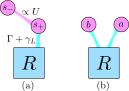
\includegraphics[width=0.6\linewidth, draft=false]{phog/entanglement_two_mode_device}
\caption{\label{fig:phog_entanglement_two_mode_device} Two-mode model of PhoG device. (a) Collective basis $s_-, s_+$, Eq.~\ref{eqn:phog_lindblad_two_mode_model}. (b) Signal basis $a, b$, Eq.~\ref{eqn:phog_two_mode_model_deriv}}
\end{figure}

However, even this symmetric system exhibiting two-photon absorption can be useful for generation of non-classical states. We will demonstrate that a symmetric PhoG device is capable to produce entanglement shared between signal modes $a$ and $b$. The system we consider is displayed in Fig.~\ref{fig:phog_entanglement_two_mode_device}. Because we wish to allow for large photon-numbers, we must resort to the linearized model described in Sec.~\ref{sec:linearization}, which allows us to access first- and second-order expectations of creation and annihilation operators. We are in a perfect position to consider the Gaussian entanglement shared between modes $a$ and $b$ \cite{Weedbrook2012, Adesso2007, Simon2000}.

We proceed as follows. After using our linearization method to solve for expectations of the form $\ev{\hat{a}}$, $\ev*{\hat{a}^\dagger \hat{a}}$, $\ev*{\hat{a}\hat{b}}$, etc., we transform these quantities into expectations of quadrature operators, Eq.~\ref{eqn:intro_quadrature}. So, for example, we form expectations as 
\begin{align}
&\ev{\hat{x}_a} = \frac{\ev{\hat{a}} + \ev{\hat{a}^\dagger}}{\sqrt{2}}, \notag \\
%
&\ev{\hat{p}_a} = \frac{i \left(\ev{\hat{a}^\dagger} - \ev{\hat{a}}\right)}{\sqrt{2}}, &\qq{etc.}\notag 
\end{align}
Crucially, we can access second-order expectations such as
\begin{align}
&\ev{\hat{x}_a \hat{x}_a} = \frac{1}{2}\left[\ev{\hat{a}^\dagger \hat{a}^\dagger} + \ev{\hat{a} \hat{a}} + 2 \ev{\hat{a}^\dagger \hat{a}} + 1\right], \notag \\
%
&\ev{\hat{x}_a \hat{p}_b} = \frac{i}{2}\left[\ev{\hat{a}^\dagger \hat{b}^\dagger} + \ev{\hat{b}^\dagger \hat{a}} - \ev{\hat{a}^\dagger \hat{b}} - \ev{\hat{a} \hat{b}} \right], \notag \\
%
&\qq{etc.} \notag
\end{align}

\noindent and therefore we can to construct a covariance matrix $\sigma$ \cite{Weedbrook2012} which describes the quadrature correlations between modes $a$ and $b$. The matrix element $\sigma_{j, k}$ is constructed as %\MT{Do I want this here? Or in the introduction?}

\begin{equation}\label{eqn:covariance matrix}
\sigma_{j, k} = \frac{1}{2} \left[ \ev{d_j d_k} + \ev{d_k d_j}\right] - \ev{d_j} \ev{d_k}
\end{equation}
with vector $\overrightarrow{d} = \left[\hat{x}_a, \hat{p}_a, \hat{x}_b, \hat{p}_b \right]$.

The Gaussian entanglement between modes $a$ and $b$ may then be calculated in terms of $\sigma_{j, k}$ via the Gaussian logarithmic negativity, $\mathcal{N}_G$ \cite{Adesso2007, Simon2000}. This entanglement measure $\mathcal{N}_G$ quantifies the extent to which the state $\rho$ described by $\sigma$ fails the positive partial transpose (PPT) criterion \cite{Simon2000, Plenio2005}. Having taken the positive partial transpose of mode $b$, $\rho \rightarrow \rho^{\text{T}_B}$, the covariance matrix transforms as
\begin{align}
&\hat{x}_a \rightarrow \hat{x}_a \notag \\
%
&\hat{p}_a \rightarrow \hat{p}_a \notag \\
%
&\hat{x}_b \rightarrow \hat{x}_b \notag \\
%
&\hat{p}_b \rightarrow - \hat{p}_b \notag
\end{align}
and we write $\tilde{\sigma}$ as this transformed covariance matrix corresponding to $\rho^{\text{T}_B}$.

\noindent The measure $\mathcal{N}_G$ is then defined as\footnote{Note the similarities between this and the logarithmic negativity \cite{Plenio2005} which is defined directly in terms of $\rho^{\text{T}_B}$.}
\begin{equation}
\mathcal{N}_G = \max\left\{0, - \log \tilde{\lambda} \right\}
\end{equation}
where $\tilde{\lambda}$ is the smallest symplectic eigenvalue of $\tilde{\sigma}$. %Make sure this is defined in the introduction

We calculate $\mathcal{N}_G$ and plot it in Fig.~\ref{fig:phog_negativities}. For example, for $\ev{\hat{a}^\dagger \hat{a}}\left(0\right) = \ev{\hat{b}^\dagger \hat{b}}\left(0\right) = 2500$, $U = 2 g$, $\gamma_c = 15 g$, $\gamma_1 = 11.5 g$ and symmetric coupling $g_a = g_b = 60 g$ (we take $g=1$), the system evolves to $\mathcal{N}_G \approx 1.25$ within $t \sim 0.01 g$, while modes $a$ and $b$ each contain approximately $18$ photons. The maximally entangled state (TMSV Eq.~\ref{eqn:intro_tmsv}) requires squeezing parameter $r = 0.62$ and thermal photon number $\bar{n} = 0.44$ to give the same $\mathcal{N}_G$, while a TMSV with $\bar{n}=18$ gives $\mathcal{N}_G = 4.3$.

 Thus, we see that the symmetric PhoG is able to generate entanglement between modes $a$ and $b$ over the intial stages of dynamics, even though it cannot produce photon-number squeezing. \MT{what is $Q$ at the same time?}


%\begin{figure}[htp]
%\centering
%\includegraphics{phog/negativities.png}
%\caption{\label{fig:phog_negativities} \MT{Can I have an inset, for example, of the photon number also? Also calculate what is $Q$.}}
%\end{figure}

\begin{figure}[htp]
\centering
	\begin{subfigure}{0.49\linewidth}
	\centering
	\includegraphics[width=\linewidth, draft=false]{phog/entanglement/entanglement_2_2}
	\caption{}
	\end{subfigure}
	\begin{subfigure}{0.49\linewidth}
	\centering
	\includegraphics[width=\linewidth, draft=false]{phog/entanglement/entanglement_3}
	\caption{}
	\end{subfigure}
	\caption{\label{fig:phog_negativities} Attainable logarithmic negativities $\mathcal{N}_G$ in the symmetric two-mode PhoG device. (a) Modes $a$ and $b$ each initialized in coherent states with $200$ photons. Symmetric coupling $g_a = g_b = 10$, $\Gamma=432$ $U=2.0$ for comparison with Fig.~\ref{fig:phog_fig3paper}. $\gamma_1 = 0$, $5$, $10$, $20$, $200$, $400$m$^{-1}$. (top to bottom). (b) Modes $a$ and $b$ each initialized in coherent states with $2500$ photons. Symmetric coupling $g_a = g_b = 60$, $\Gamma = 1087$, $gamma_1 = 0$, $5$, $11.5$, $20$, $200$, $400$m$^{-1}$. $U = 2.0$.}
\end{figure}


\section{Outlook}
In this chapter, we have introduced and analysed a device, which we denote \emph{PhoG}, which is capable to produce highly non-classical states at the output, with just a coherent state at the input. Depending on whether the device is configured with asymmetric signal mode coupling (Secs.~\ref{sec:phog_single_mode_model}-\ref{sec:phog_multi_mode}) or symmetric signal mode coupling (Sec.~\ref{sec:phog_entanglement}) the device produces either a strongly photon-number squeezed (sub-Poissonian) state, or an entangled state. In the limit of no linear loss, $\gamma_1 \rightarrow 0$ the sub-Poissonian output of the asmmetric PhoG tends towards a single-photon Fock state. However, even with realistic loss and realistic levels of nonlinearity, the device is predicted to create bright output states which are strongly sub-Poissonian, with feasible predicted Mandel parameter $Q \gtrsim -0.8$.

The device relies on realising an exotic form of dissipation, known as Nonlinear Coherent Loss (NCL), and which is simulated in our realistic multi-mode system via strong linear loss (realised by the waveguide "tail") and Kerr nonlinearity. Our hierarchy of models agree in their observation of the two key behaviours of NCL and so we are confident that $Q < 0$ should be observable in a full, finished device. Our design of the PhoG device with a system of waveguides laser-inscribed into bulk IG$2$ glass should serve as a practical design for deterministic sources of non-classicality. Since the glass is comparatively inexpensive, the device itself relatively easy to produce, and coherent states are deemed a "cheap" quantum state to use, the PhoG device can find applications in several different imaging, measurement and metrology tasks \cite{Taylor2013, Ruo2019}. \MT{Do I want to add some chat about its use for imaging in the setup from supertwin?}

We desire to undertake further modelling of the realistic multimode PhoG device described in Sec.~\ref{sec:phog_multi_mode}, in order to relax several simplifying assumptions which we have made in this chapter. The assumption made in Sec.~\ref{sec:parameters} that the pulse shape is unchanging over the course of evolution seems unrealistic in a realistic system in which linear (evanescent) coupling, self-phase modulation and dispersion are all present. It should therefore be directly verified what impact the inclusion of these effects has in a system where the pulse shape is permitted to change. Furthermore, the pulse durations of approx $100$~fs considered in this Chapter are on the threshold for when higher-order effects such as Raman scattering should be considered.

We have recently begun some preliminary work on this question% and believe we have good evidence that NCL will be evidenced even in such a system when the pulse envelope is directly modelled. 
. In particular, we have begun investigating the spectral and temporal properties of a pulse in a system identical to the multi-mode one, Sec.~\ref{sec:phog_multi_mode}, including chromatic dispersion, self-phase modulation and self-steepening. We solve the so-called nonlinear Schr{\"o}dinger equation (NLSE):

\begin{equation}\label{eqn:phog_nlse}
\frac{\partial A_j}{\partial z} + i \beta_1 \frac{\partial A_j}{\partial \tau} _ i \frac{\beta_2}{2} \frac{\partial^2 A_j}{\partial \tau^2} - \frac{\beta_3}{6} \frac{\partial^3 A_j}{\partial \tau^3} + \frac{\gamma_1}{2} = i \gamma_{NL} \left( 1 + \frac{i}{\omega_0} \frac{\partial}{\partial \tau}\right)\left|A_j\right|^2 A_j - i g_{j, k} A_k
\end{equation}
where $A_j\left(z, \tau\right)$ is the pulse envelope in the $j^{\text{th}}$ waveguide, $\gamma_1$ is the linear loss parameter, $\gamma_{NL}$ is the nonlinearity parameter given by
\begin{equation}
\gamma_{NL} = \frac{n_2 \omega_0}{c A_{\text{eff}}},
\end{equation}
$\omega_0$ is the carrier frequency of the pulse, $g_{j, k}$ describes coupling between waveguide $j$ and waveguide $k$, and the $\beta$ are the first-, second-, and third-order dispersion terms. The propagation direction is $z$ and this equation is valid in a frame co-moving with the pulse, with intra-pulse coordinate $\tau$. This equation may be solved via the split-step Fourier method \cite{Agrawal2007}.

One should note that Eq.~\ref{eqn:phog_nlse} is an entirely classical equation describing the evolution of the pulse's envelope $A$, and so cannot give us direct information about quantum effects such as the photon-number statistics or entanglement properties. However an observation of NL decay of the pulse energies contained within the signal modes should be possible and we will take such an observation as a hopeful signature that NCL may indeed be present.

There are several methods which may be used to quantize Eq.~\ref{eqn:phog_nlse}, such as the back-propagation method \MT{cite} or \MT{the other one.} An immediate next-step will be to employ either of these methods and check whether we indeed observe a Mandel parameter $Q < 0$. The method \MT{X} has been successfully applied to similar systems and it has been observed \MT{cite} that a similar setup can induce spectral entanglement within the pulse. If this can be observed for our PhoG device it will be another proof of its versatility to generate a broad array of nonclassical behaviours, deterministically from a quasi-classical input.









